\documentclass[a4paper]{cernatsnote}
\usepackage[utf8]{inputenc}

\usepackage{subcaption}
\usepackage{graphicx}
\usepackage{longtable}
\usepackage{booktabs}
\usepackage{float}
\usepackage{comment}

\title{Injection optics commissioning in 2021 and 2022}
\documentlabel{CERN-ACC-NOTE-2022-YYYY}
\keywords{optics, LHC, beam-test}

\author{ T.~Persson, J.~Dilly, S.~Faroukh, E.~Fol, H.~Garc\'ia Morales, M.~Hofer,
 J.~Keintzel, M.~Le~Garrec, E.H.~Maclean, L.~Malina,  F.~Soubelet, R.~Tom\'as, L.~Van~Riesen-Haupt,  A.~Wegscheider}
\date{December 2022}
%Plots to include:
%comp with old Vertical dispersion
%Comp with old measurement beta-beat
%Second order dispersion
%3D kicks ?
\begin{document}
\maketitle
\begin{abstract}
The LHC Run~3 injection optics commissioning started with the beam test in 2021 and was finalized in 2022.
The beam test aimed at finding potential issues with the machine, testing the new software and hardware and progressing with the general commissioning in view of the full restart in 2022.
First optics measurements at injection energy revealed a significantly larger $\beta$-beating than in Run~2.
This document describes the commissioning steps to fully correct and validate the LHC injection optics.


\end{abstract}

\section{The Run 3 injection optics}
The injection optics deployed in Run 3 is almost identical to the injection optics in the second half of Run~2 after deploying the ATS optics~\cite{ats_stephane}.
During Long Shutdown 2 (LS2) it was decided to remove one warm quadrupole on either side of IP7, MQWA.E5, to replace them with shielding and keep the magnets as spares~\cite{roderik}. The IR7 optics was rematched to
keep it as similar as possible to the Run~2 optics. Figure~\ref{fig:IR7} shows the IR7 optics both for Run 2 and Run~3. 

During LS2 various LHC magnets were exchanged~\cite{LS2,LS2a}:
19 LHC dipoles,
3 arc quadrupoles, one IR quadrupole (RQTL7.R3) and various dipole spool pieces (sextupolar, octupolar and decapoar).
Furthermore, 2 new sextupoles and two additional octupoles were also installed.
In principle, these changes should not affect the optics.

A general description of the Run~3 optics can be found in~\cite{run3}.


\begin{figure}
\begin{subfigure}{1.\textwidth}
  \centering
  % include first image
  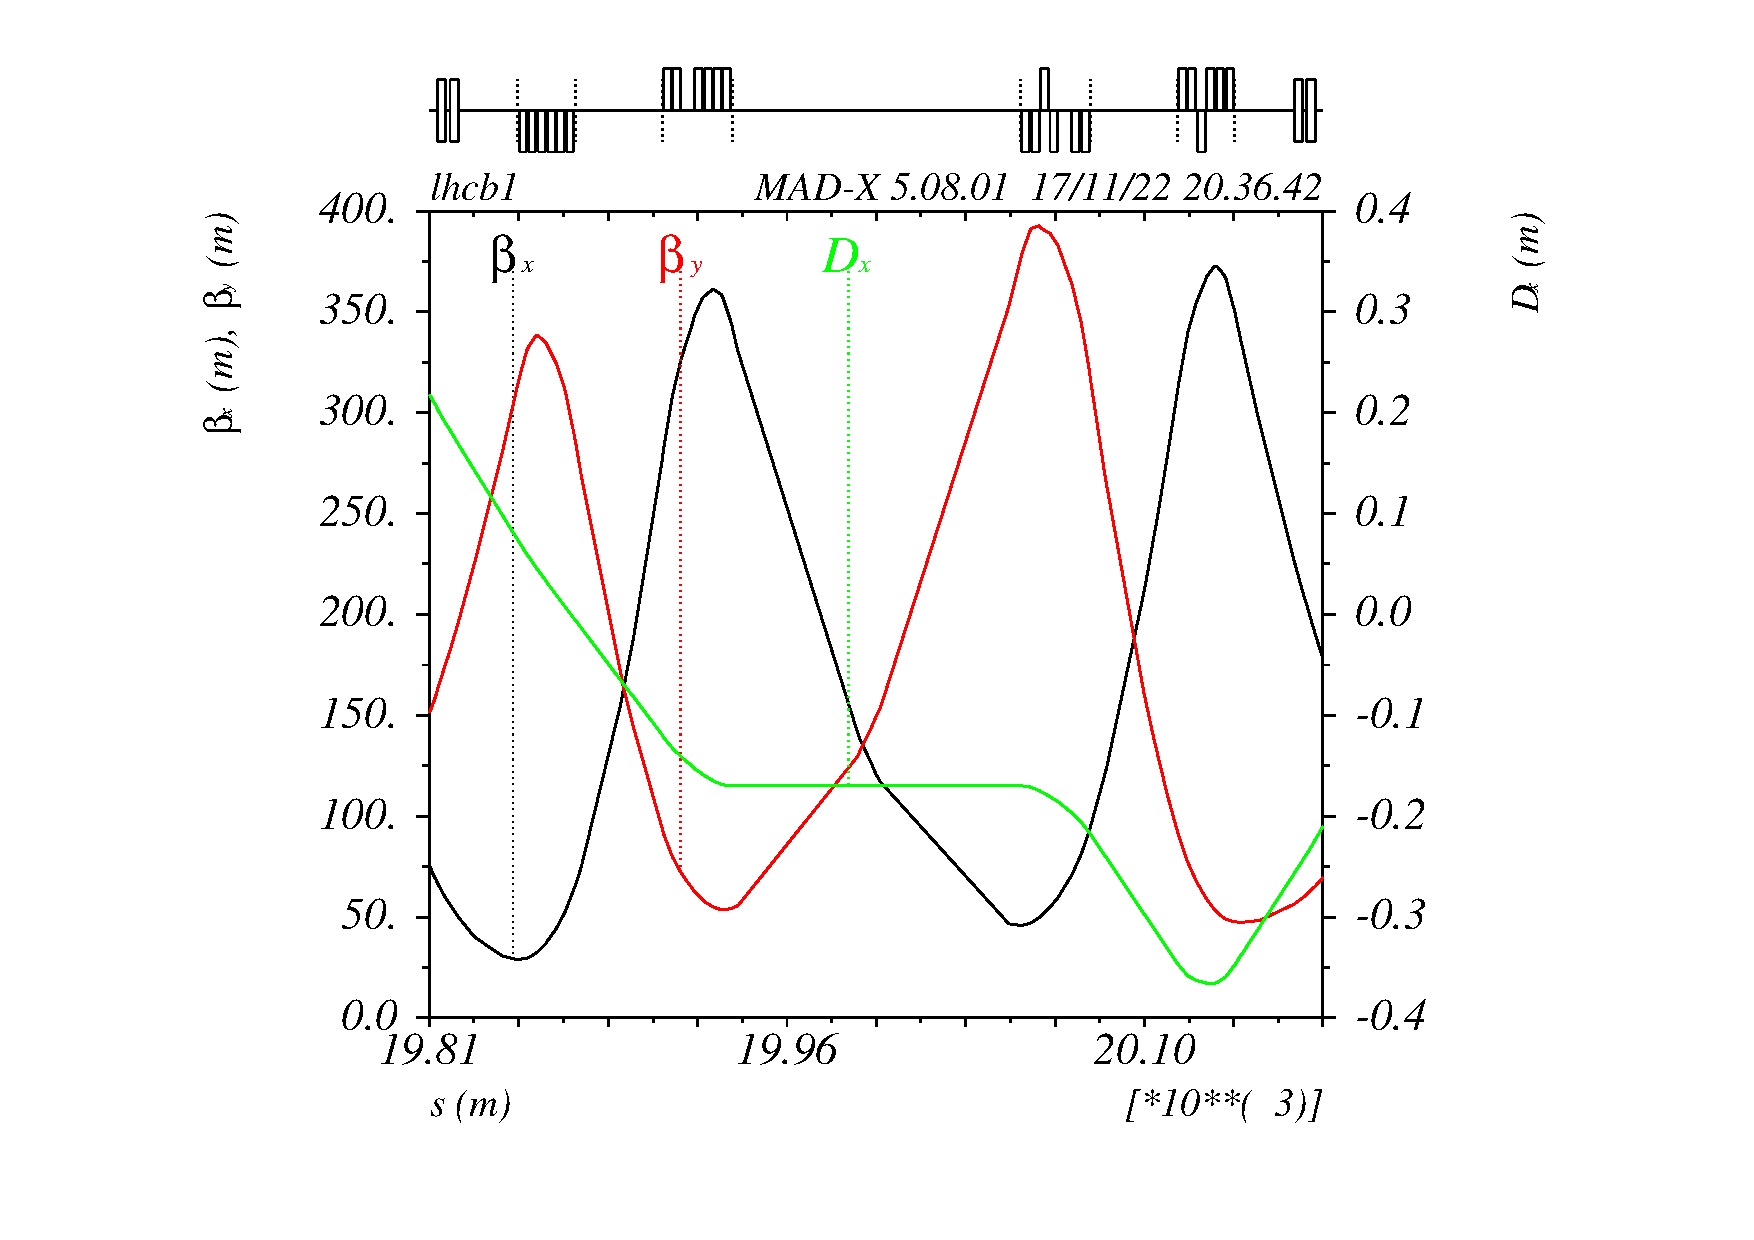
\includegraphics[width=0.76\linewidth, trim=85 45 70 15, clip]{plots/beam1/IR7_Run2.pdf}  
  \caption{Run 2}
\end{subfigure}
\begin{subfigure}{1.\textwidth}
  \centering
  % include second image
  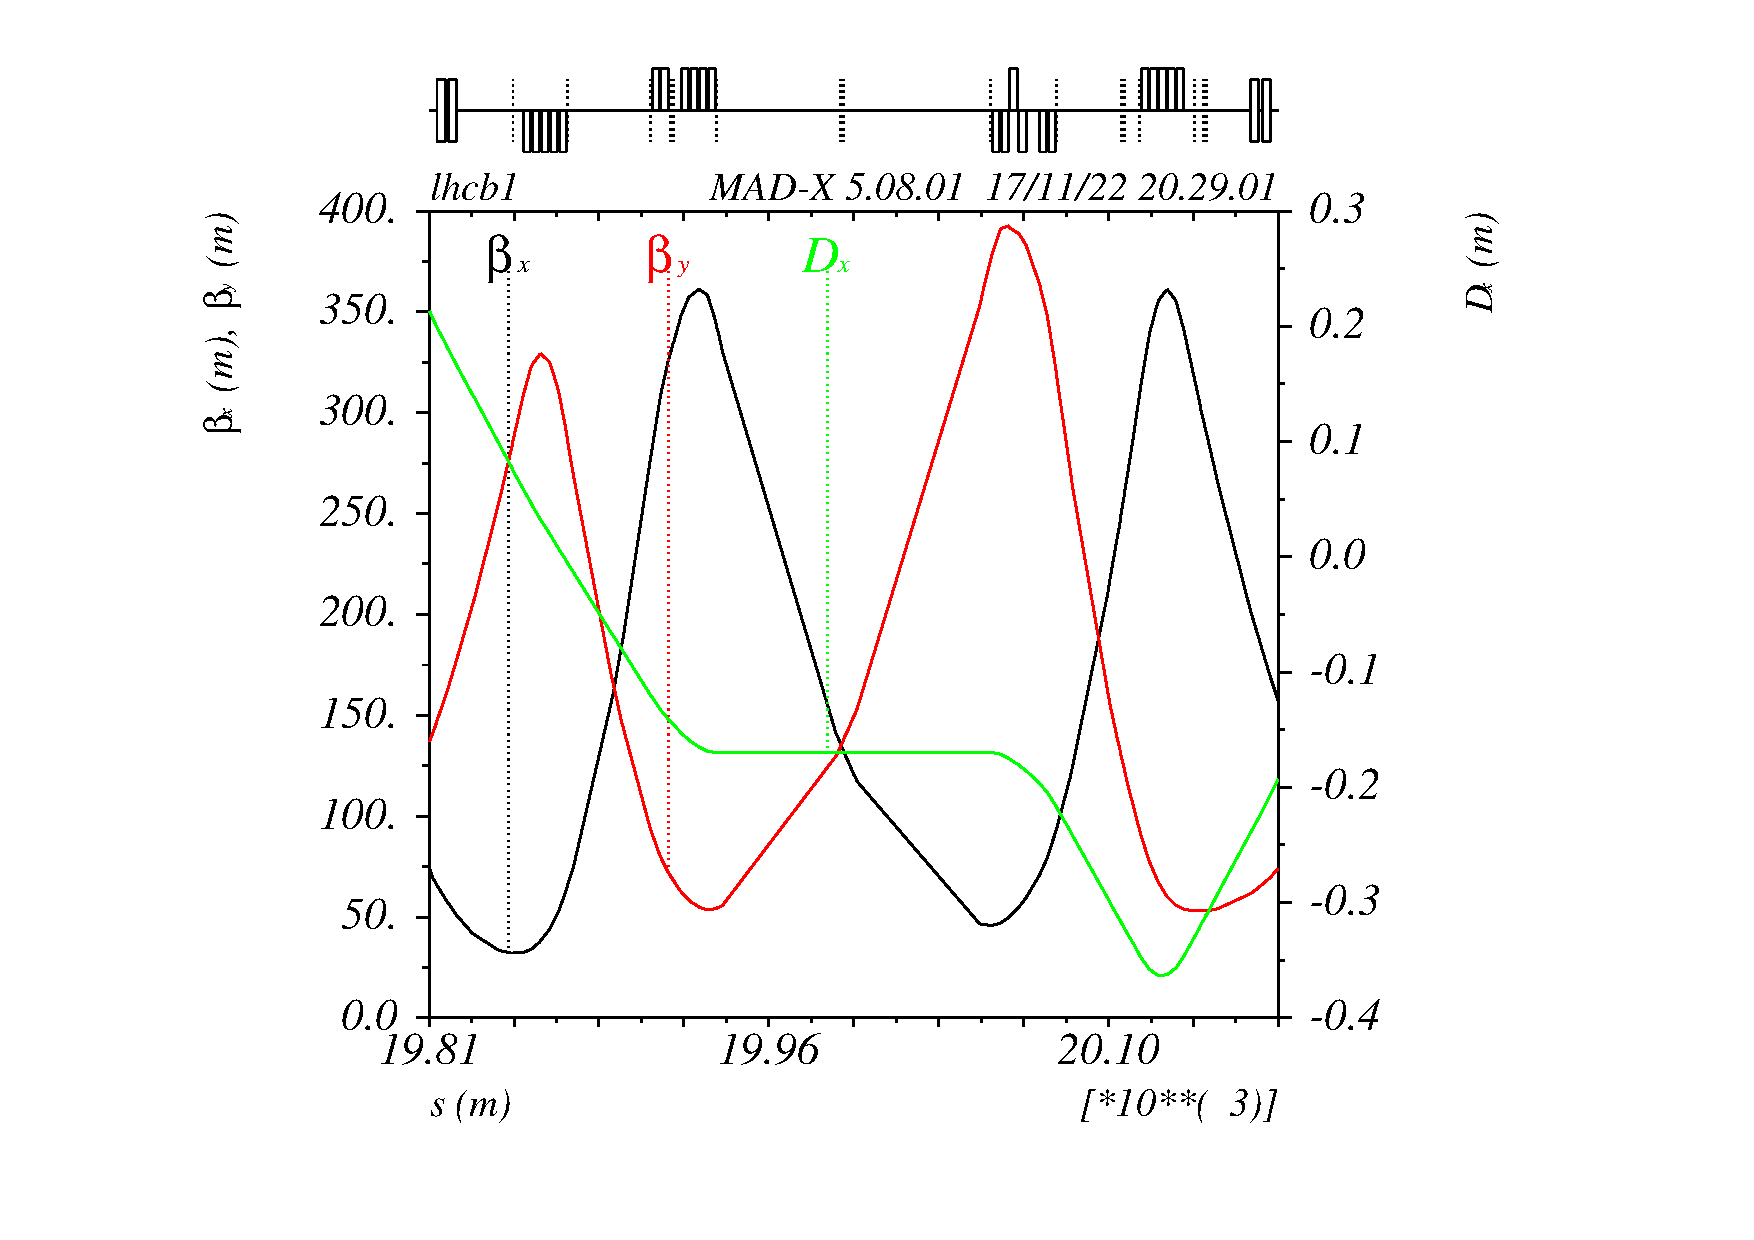
\includegraphics[width=.83\linewidth, trim=65 45 70 15, clip]{plots/beam1/IR7_Run3.pdf}  
  \caption{Run 3}
\end{subfigure}
\caption{IR7 layout and Beam 1 optics for Run~2 and Run~3. The rightmost and leftmost quadrupole blocks (Q5) have one fewer MQW (5 instead of 6) in Run 3 with a negligible impact on the optics functions.}
\label{fig:IR7}
\end{figure}


\section{Linear optics commissioning}
The beam test week took place in the autumn of 2021 with the intention of testing the LHC after the Long Shutdown~2 (LS2) to be ready for the full restart in 2022.
The initial measurement of the $\beta$-beating showed significantly higher values than what was measured in Run~2 during commissioning. This is shown in Fig.~\ref{fig:initalVs2016} for Beam~1 and Beam~2.  


\begin{figure}[ht]
\begin{subfigure}{.5\textwidth}
  \centering
  % include first image
  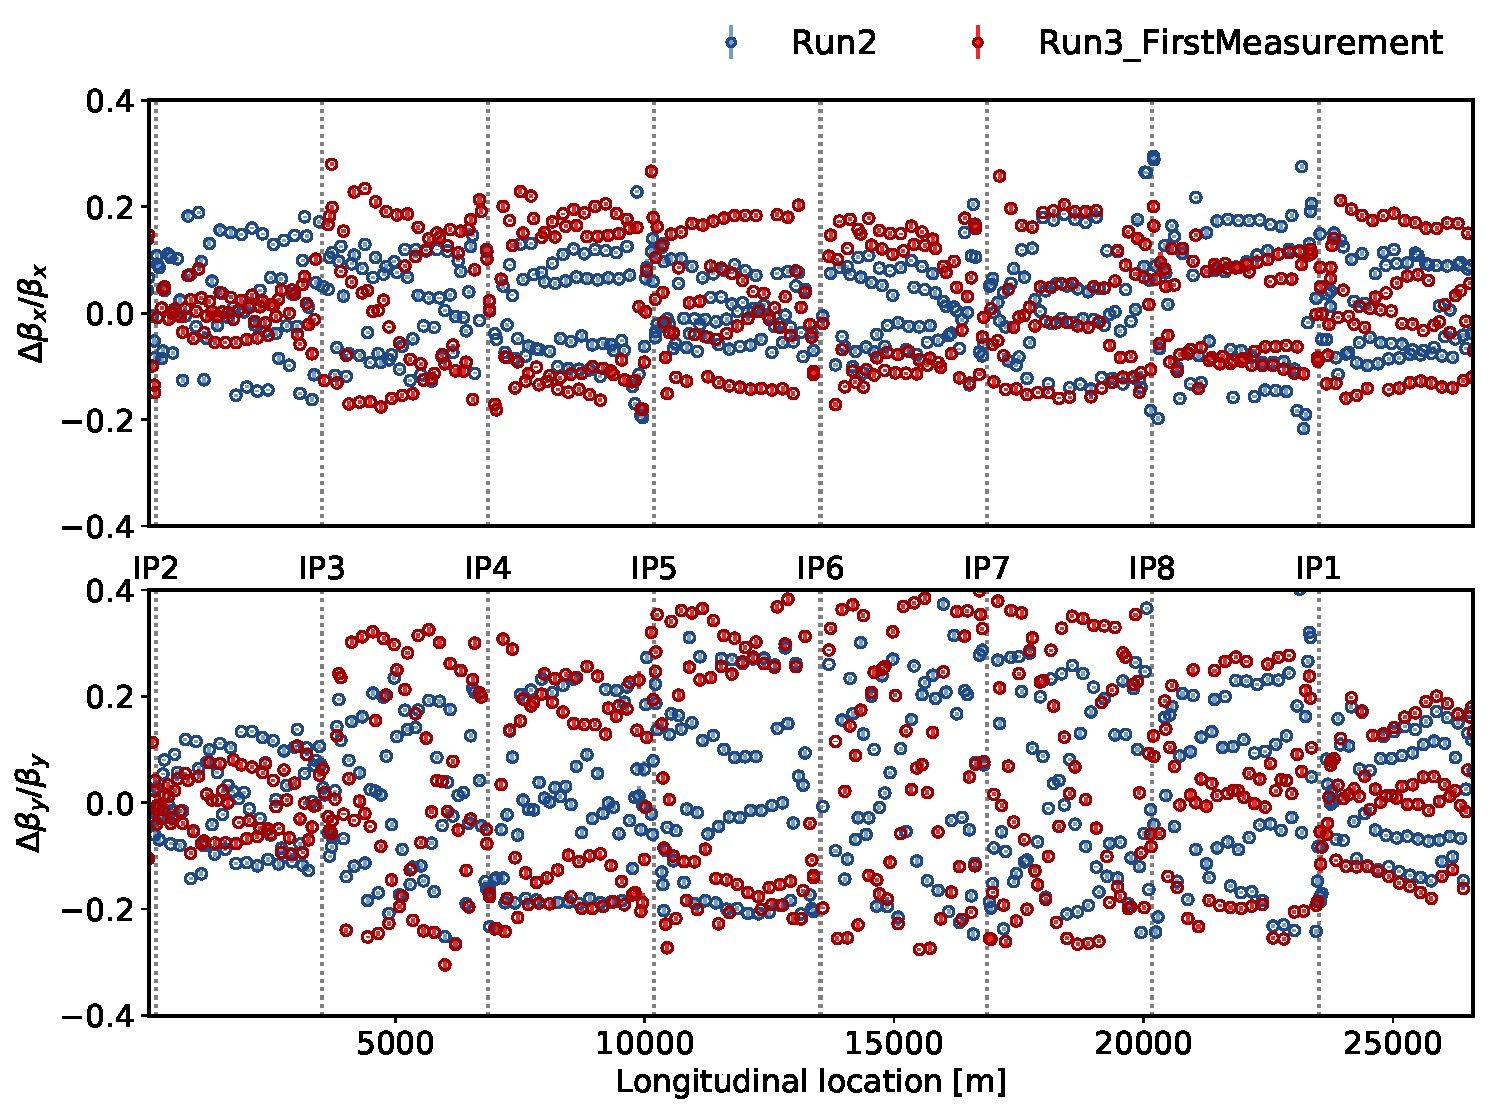
\includegraphics[width=.99\linewidth]{plots/beam1/beta_beat_virgin_2016_2021.pdf}  
  \caption{Beam~1}
\end{subfigure}
\begin{subfigure}{.5\textwidth}
  \centering
  % include second image
  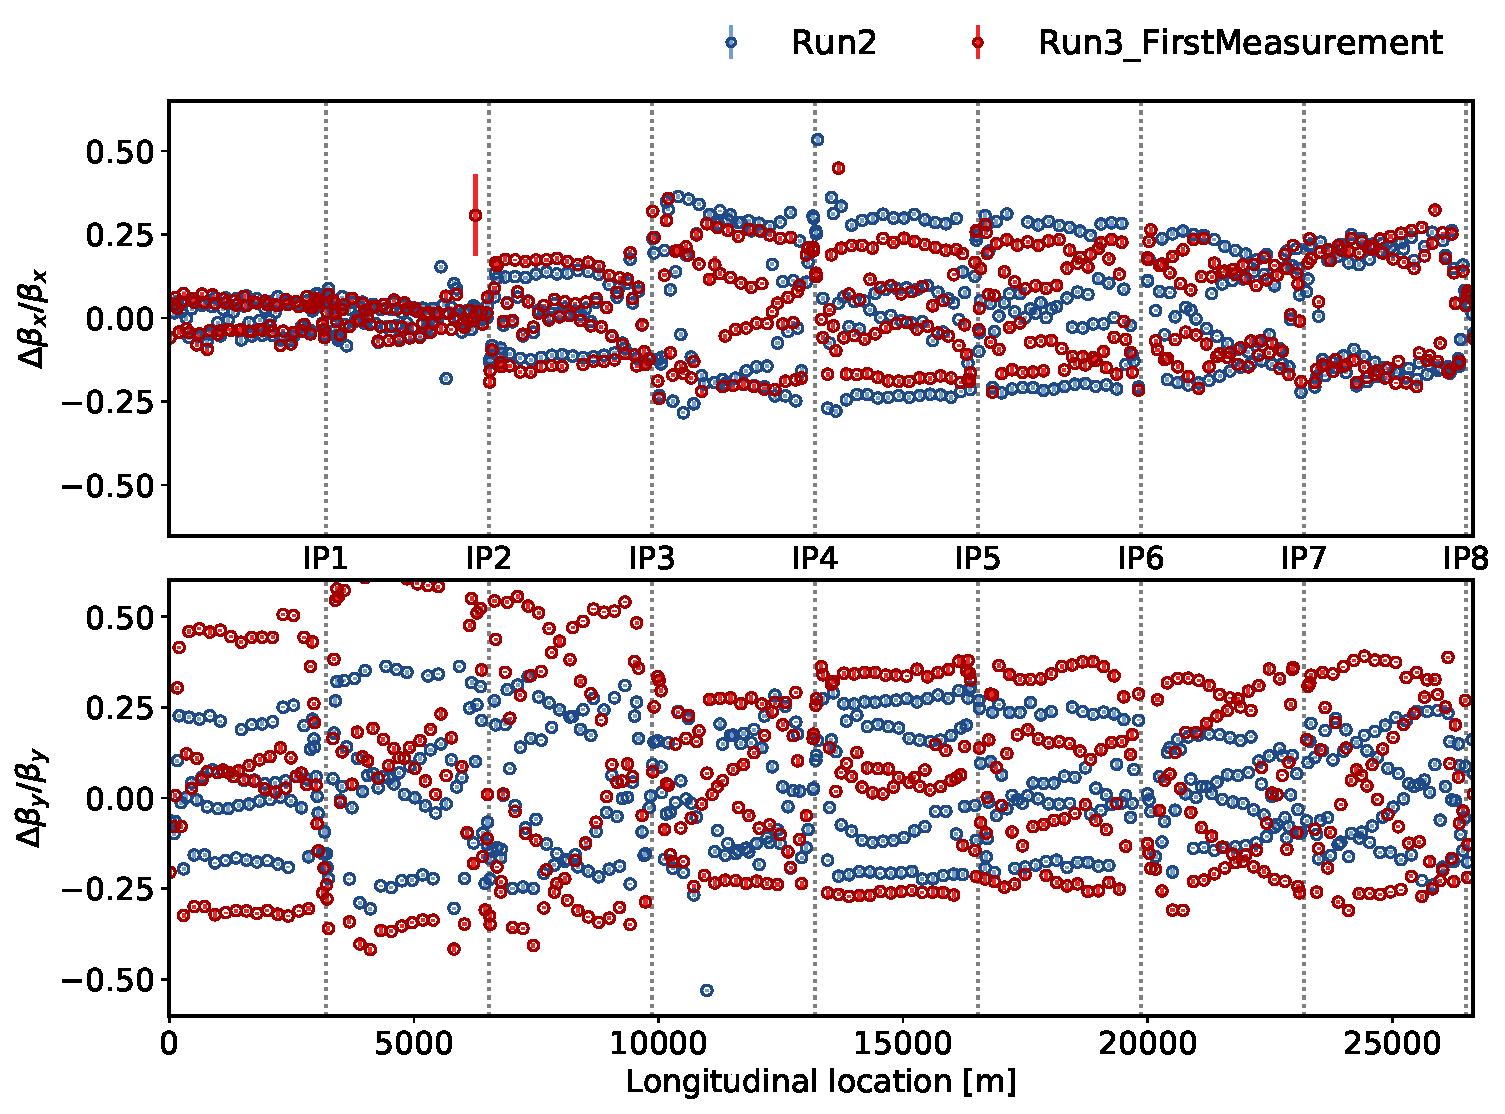
\includegraphics[width=.99\linewidth]{plots/beam2/B2_BetaBeat_2016_vs_first2021.pdf}  
  \caption{Beam~2}
\end{subfigure}
\caption{The $\beta$-beating for the first measurement in 2021 compared to the measurement in 2016 (during MD) showing a significantly larger $\beta$-beating in 2021, specially in the Beam~2 vertical plane.}
\label{fig:initalVs2016}
\end{figure}
%beta_beat_before_after_pre_beam1.pdf

To identify the source of this discrepancy it was first decided to perform a magnetic cycle of the machine since the machine had been at injection energy for about 40~hours. Figure~\ref{fig:before_after_pre_cycle} compares the $\beta$-beating after 40 hours at injection and right after a magnetic ecycle, showing a small difference of only few percent. This is a positive result since it allows to have long fills at injection. 

\begin{figure}[ht]
\begin{subfigure}{.5\textwidth}
  \centering
  % include first image
  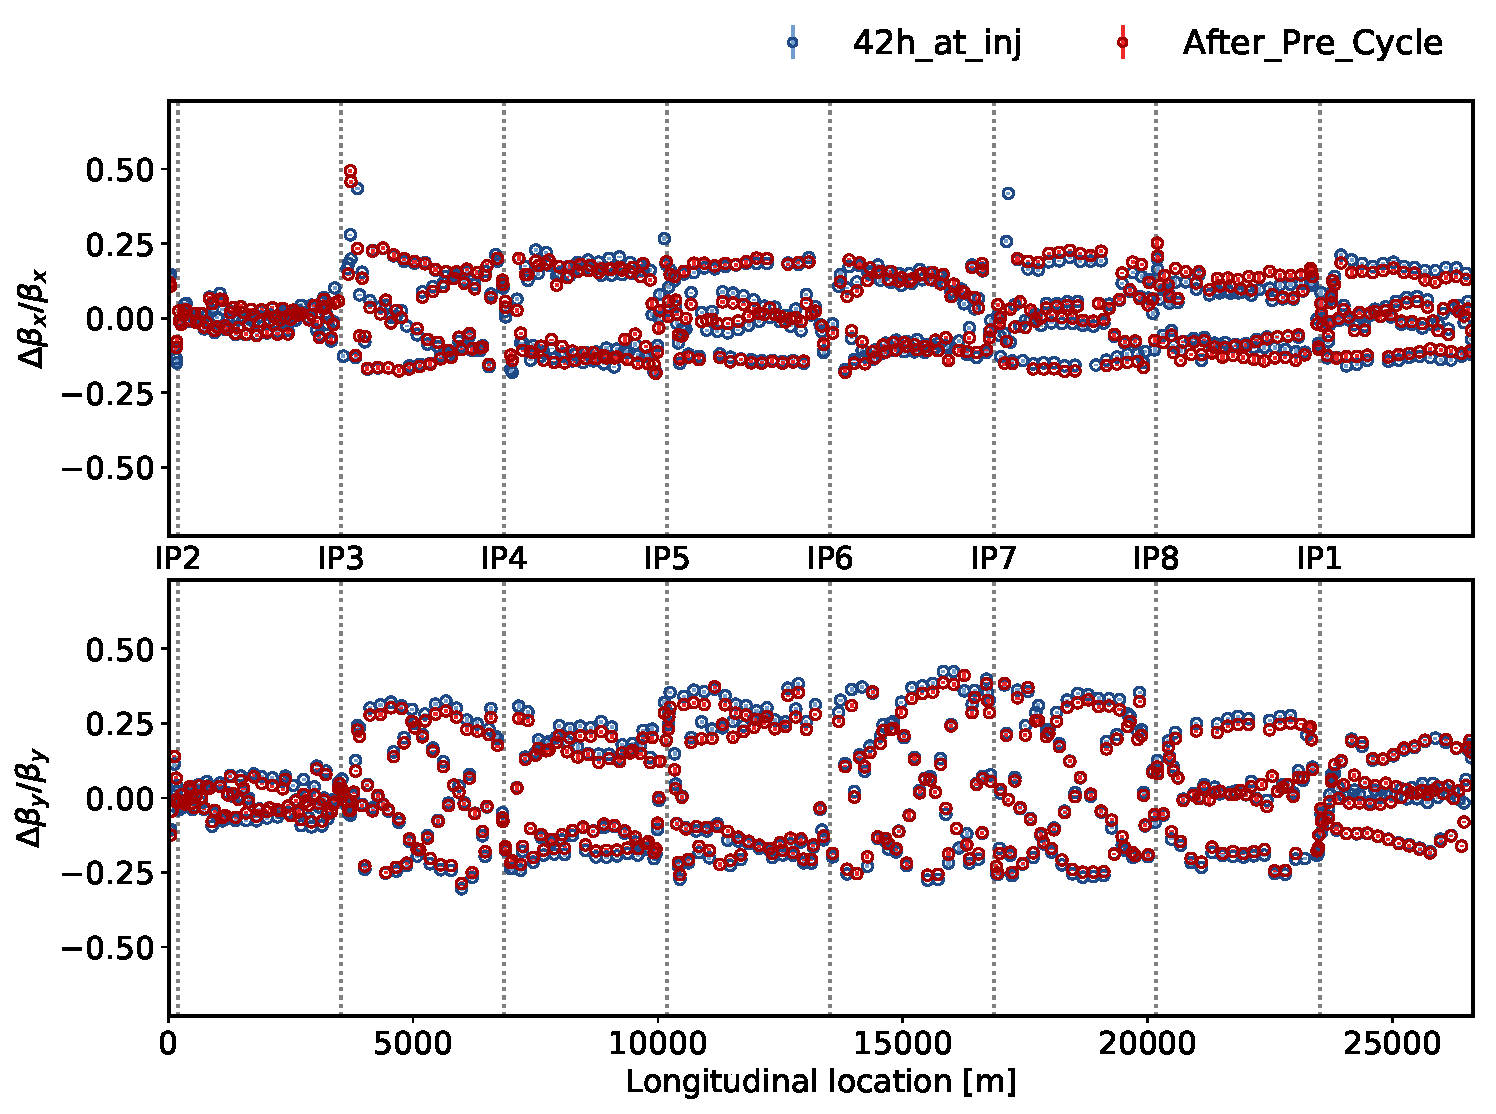
\includegraphics[width=.99\linewidth]{plots/beam1/beta_beat_before_after_pre_beam1.pdf}  
  \caption{Beam~1}
\end{subfigure}
\begin{subfigure}{.5\textwidth}
  \centering
  % include second image
  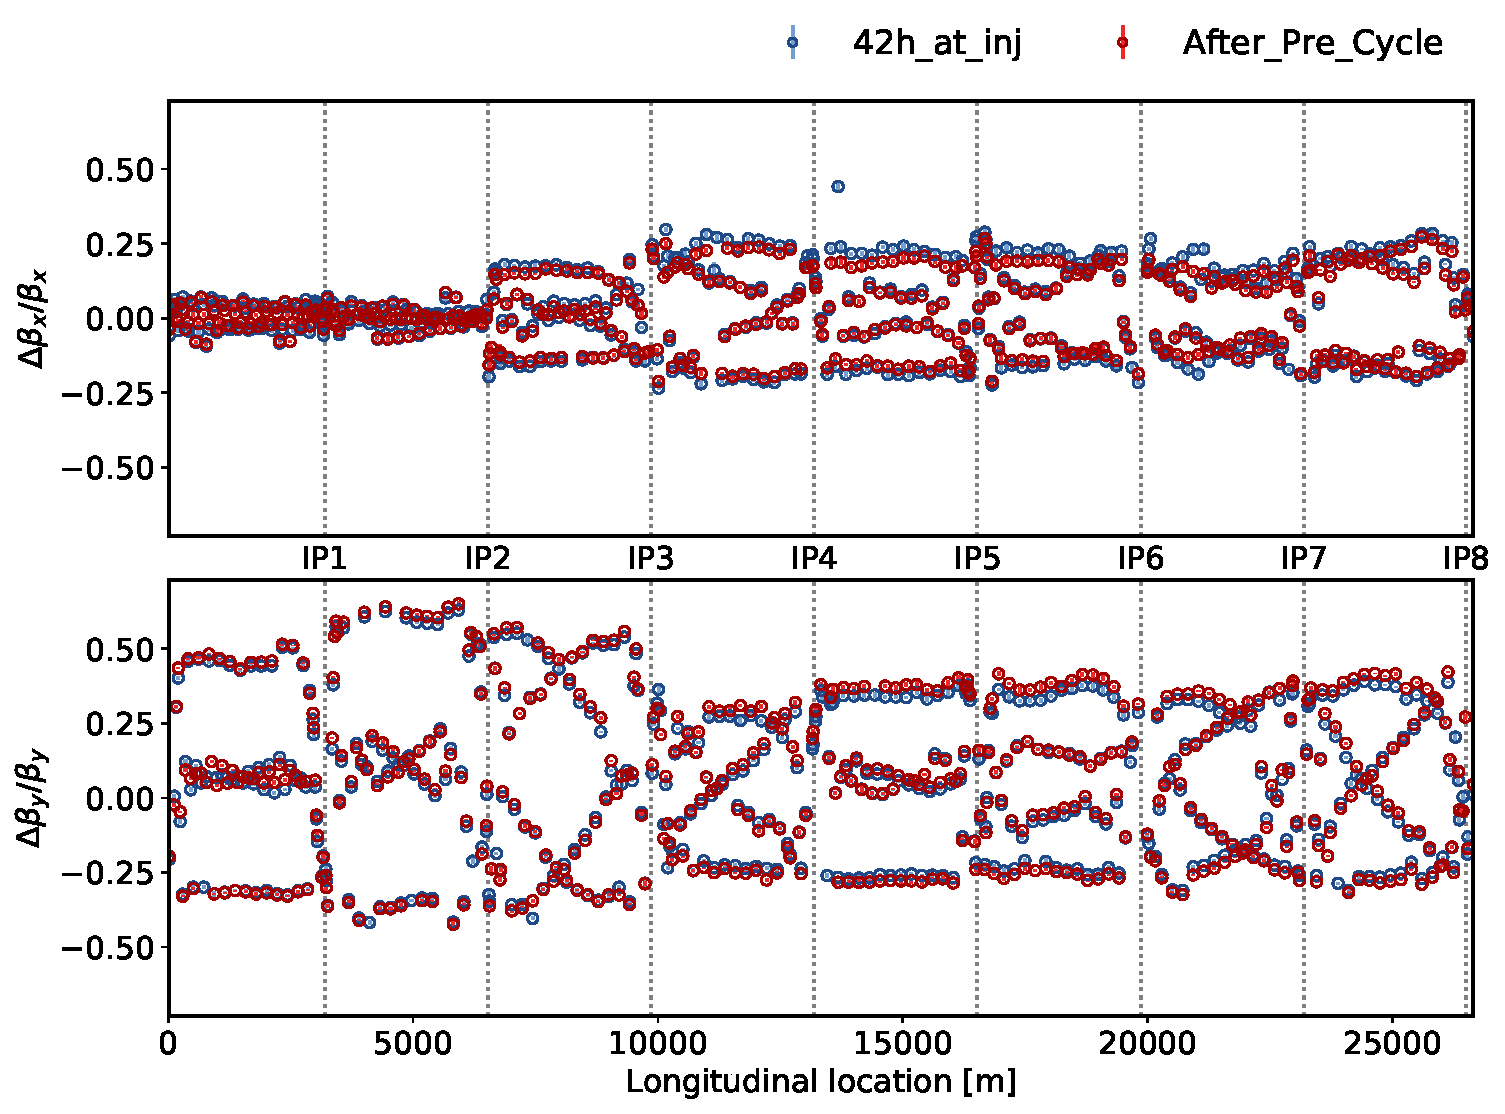
\includegraphics[width=.99\linewidth]{plots/beam2/beta_beat_before_after_pre_beam2.pdf}  
  \caption{Beam~2}
\end{subfigure}
\caption{A comparison of the $\beta$-beating right after precycling and after 42~hours at injection showing a difference within 2-3\%.}
\label{fig:before_after_pre_cycle}
\end{figure}


After ruling out that the big change in $\beta$-beating was coming coming from the extended time spent at injection we attempted to find the location of the error. Using the Segment-by-Segment (SbS)~\cite{first} technique it was found that there was a large phase deviation around IP3 and in particular at RQTL7.R3.B2. An optics correction using only this magnet was computed. The first observation was that nothing changed at all, not even the tunes, in Beam~2. However, the tune was changing for Beam 1. Therefore the RQTL7.R3.B1 and RQTL7.R3.B2 power converters were swapped. This was then traced to an old swap already detected in Run~1. This was fixed at that time but then during the LS2 it was again re-introduced as this magnet was replaced~\cite{first, michiEvian}. This swap was corrected on the software side and a new measurement was carried out showing a significantly reduced $\beta$-beating, see~Fig.~\ref{fig:before_after_swap}.

\begin{figure}[ht]
\begin{subfigure}{.5\textwidth}
  \centering
  % include first image
  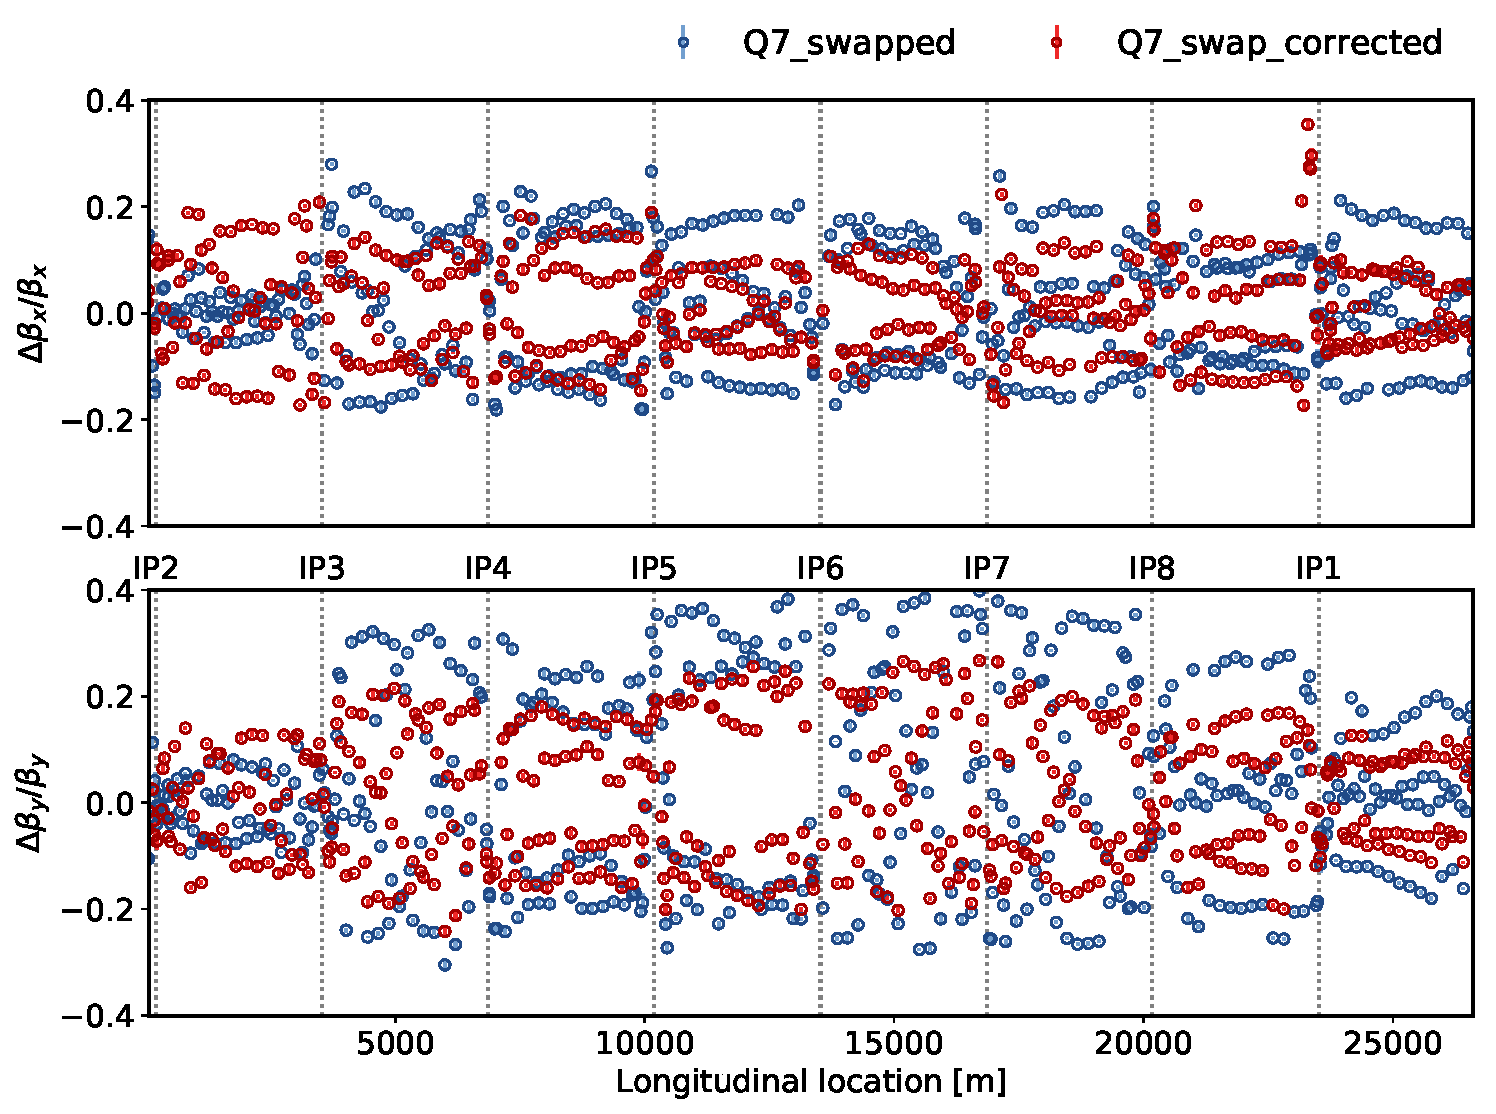
\includegraphics[width=.99\linewidth]{plots/beam1/beta_beat_before_after_swap.pdf}  
  \caption{Beam~1}
\end{subfigure}
\begin{subfigure}{.5\textwidth}
  \centering
  % include second image
  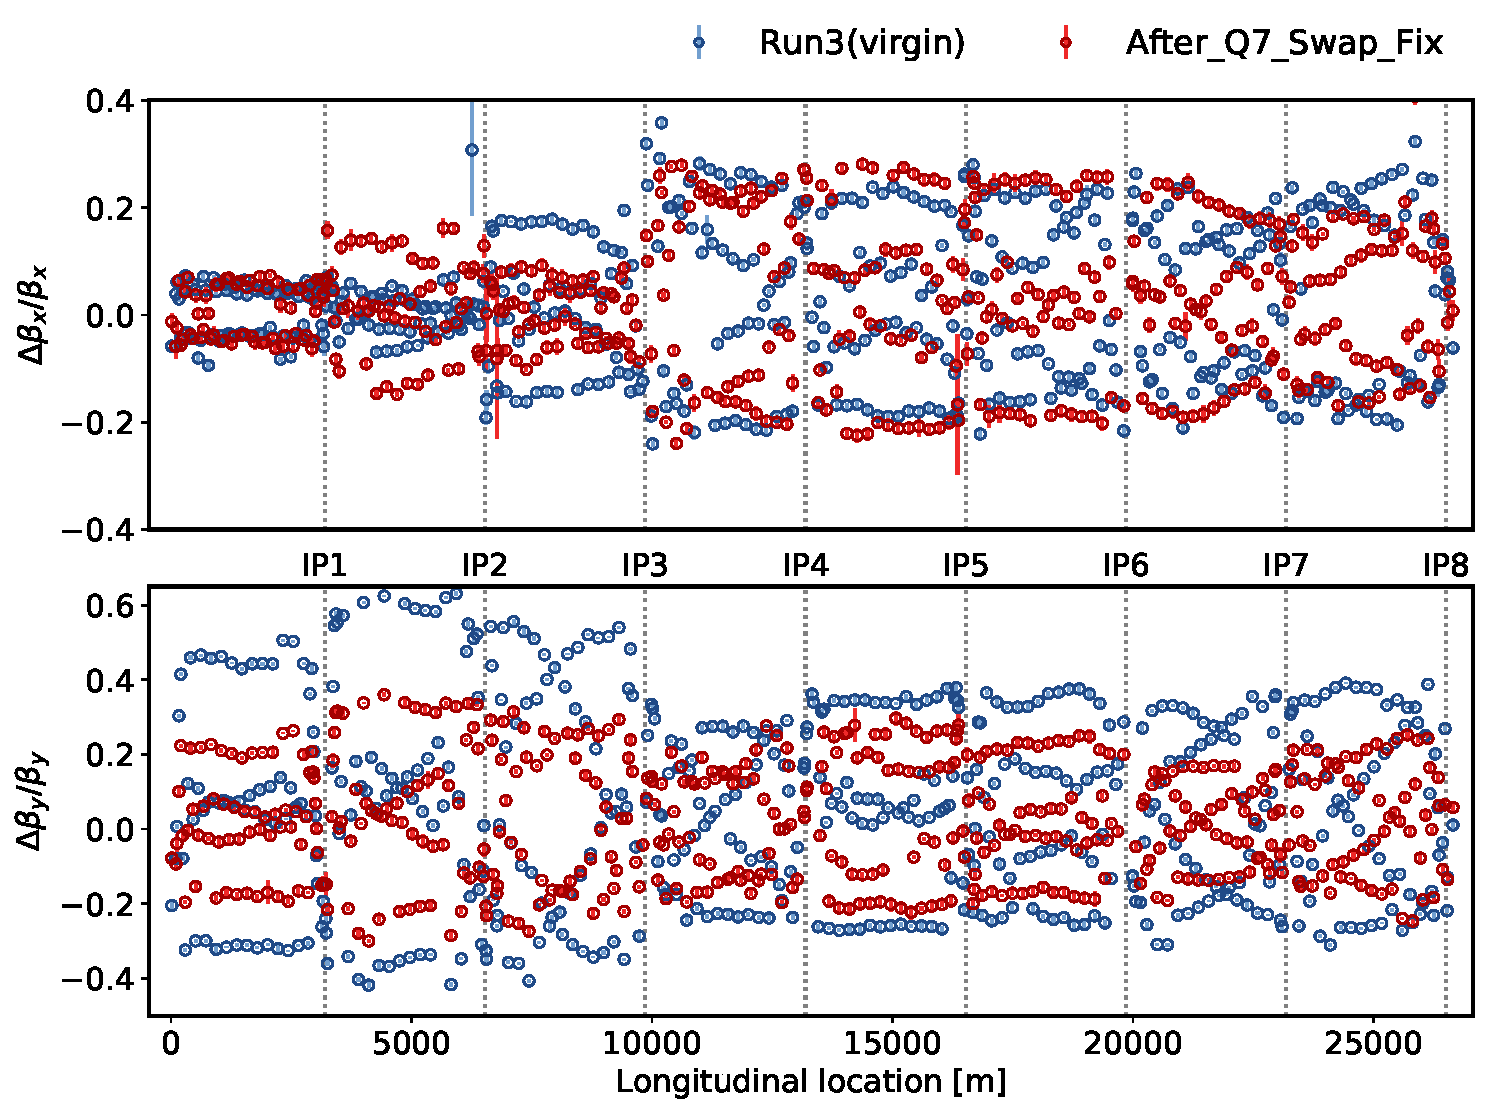
\includegraphics[width=.99\linewidth]{plots/beam2/beta_beat_before_vs_after_Q7_swap.pdf}  
  \caption{Beam~2}
\end{subfigure}
\caption{A comparison of the $\beta$-beating before and after correcting the Beam~1 and Beam~2 power converter swap of the RQTL7.R3 magnet.}
\label{fig:before_after_swap}
\end{figure}

Figure~\ref{fig:after_swap_vs_2016} shows a comparison of the $\beta$-beating between Run~2 and Run~3 (after the power converter swap) with differences below 10\%. This difference could be partly explained by the different field quality of the dipoles and quadrupoles that were exchanged during LS2~\cite{LS2} plus the intrinsic optics fluctuations studied in Section~\ref{sec:repro}. 

\begin{figure}[ht]
\begin{subfigure}{.5\textwidth}
  \centering
  % include first image
  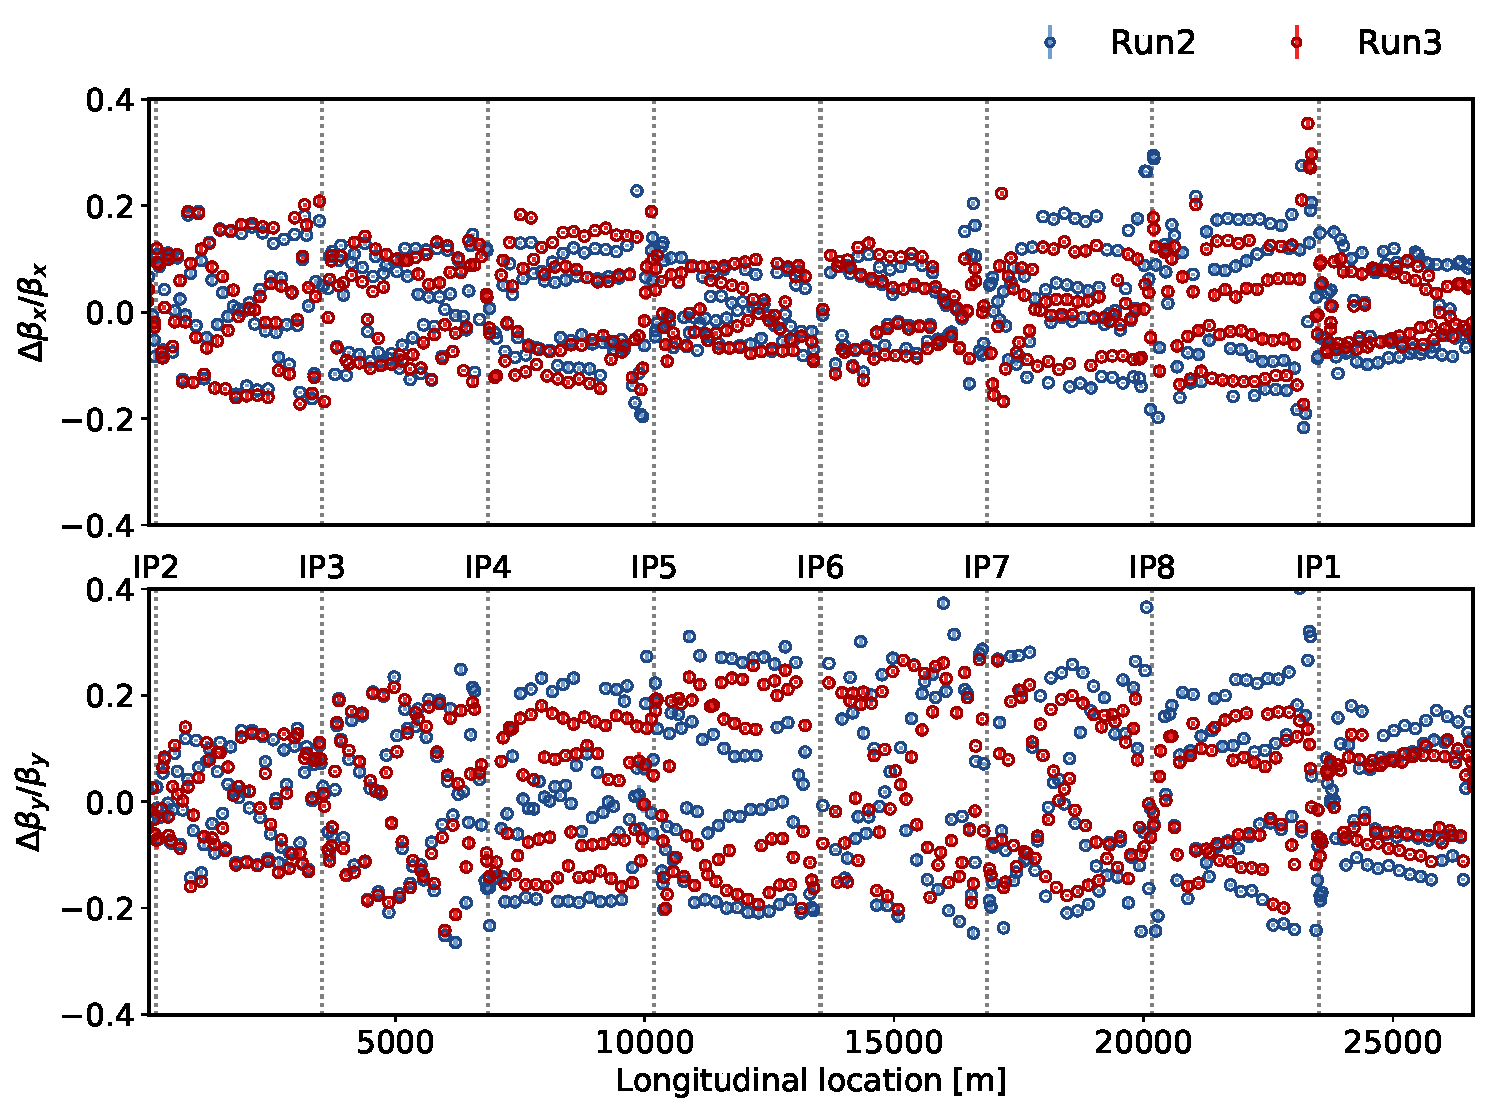
\includegraphics[width=.99\linewidth]{plots/beam1/beta_beat_2016_2021_swap_fixed.pdf}   
  \caption{Beam~1}
\end{subfigure}
\begin{subfigure}{.5\textwidth}
  \centering
  % include second image
  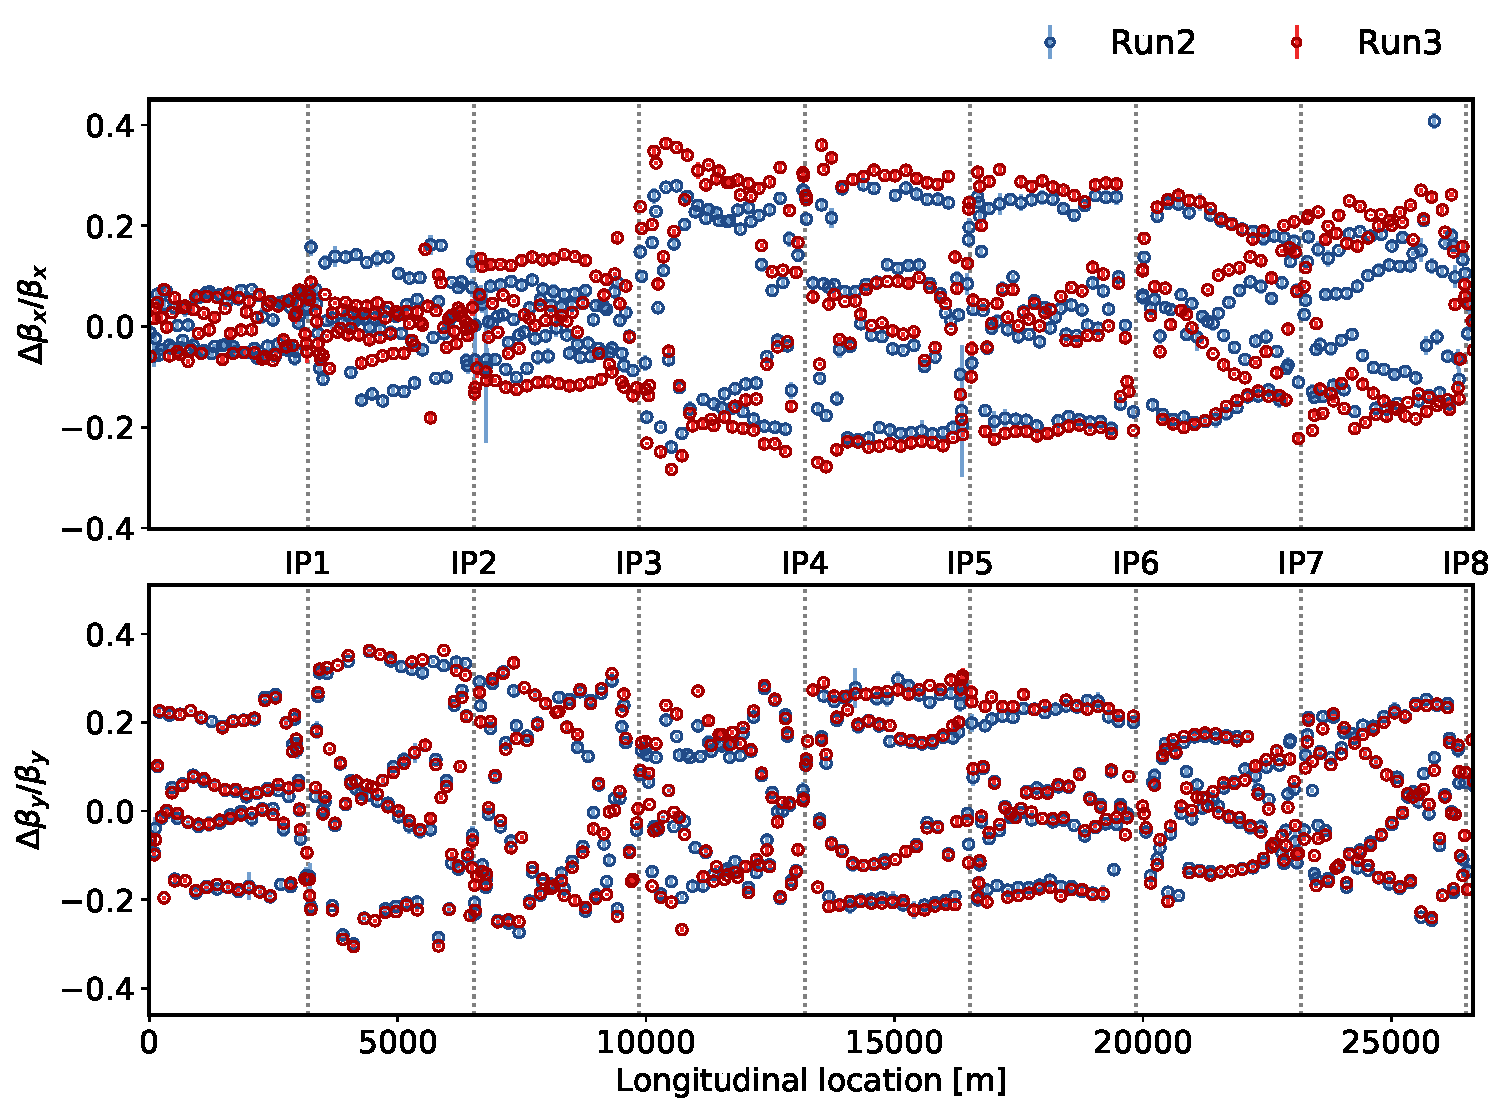
\includegraphics[width=.99\linewidth]{plots/beam2/B2_BetaBeat_afterIR3Q7fix_vs_virgin2016.pdf}
  \caption{Beam~2}
\end{subfigure}
\caption{Comparison of the $\beta$-beating between Run~2 and Run~3 virgin machines (after the fix of RQTL7.R3).}
\label{fig:after_swap_vs_2016}
\end{figure}

Based on the measurement after the correction of the swapped quadrupole, a global correction of the phase advance as well as the normalized horizontal dispersion was calculated. The impact on the $\beta$-beating is shown in Fig.~\ref{fig:before_after_correction_beta_beat} and the effect on the normalized dispersion is shown in Fig.~\ref{fig:before_after_correction_ndisp}. This was done without crossing angles and separtion bumps. 

\begin{figure}[ht]
\begin{subfigure}{.5\textwidth}
  \centering
  % include first image
  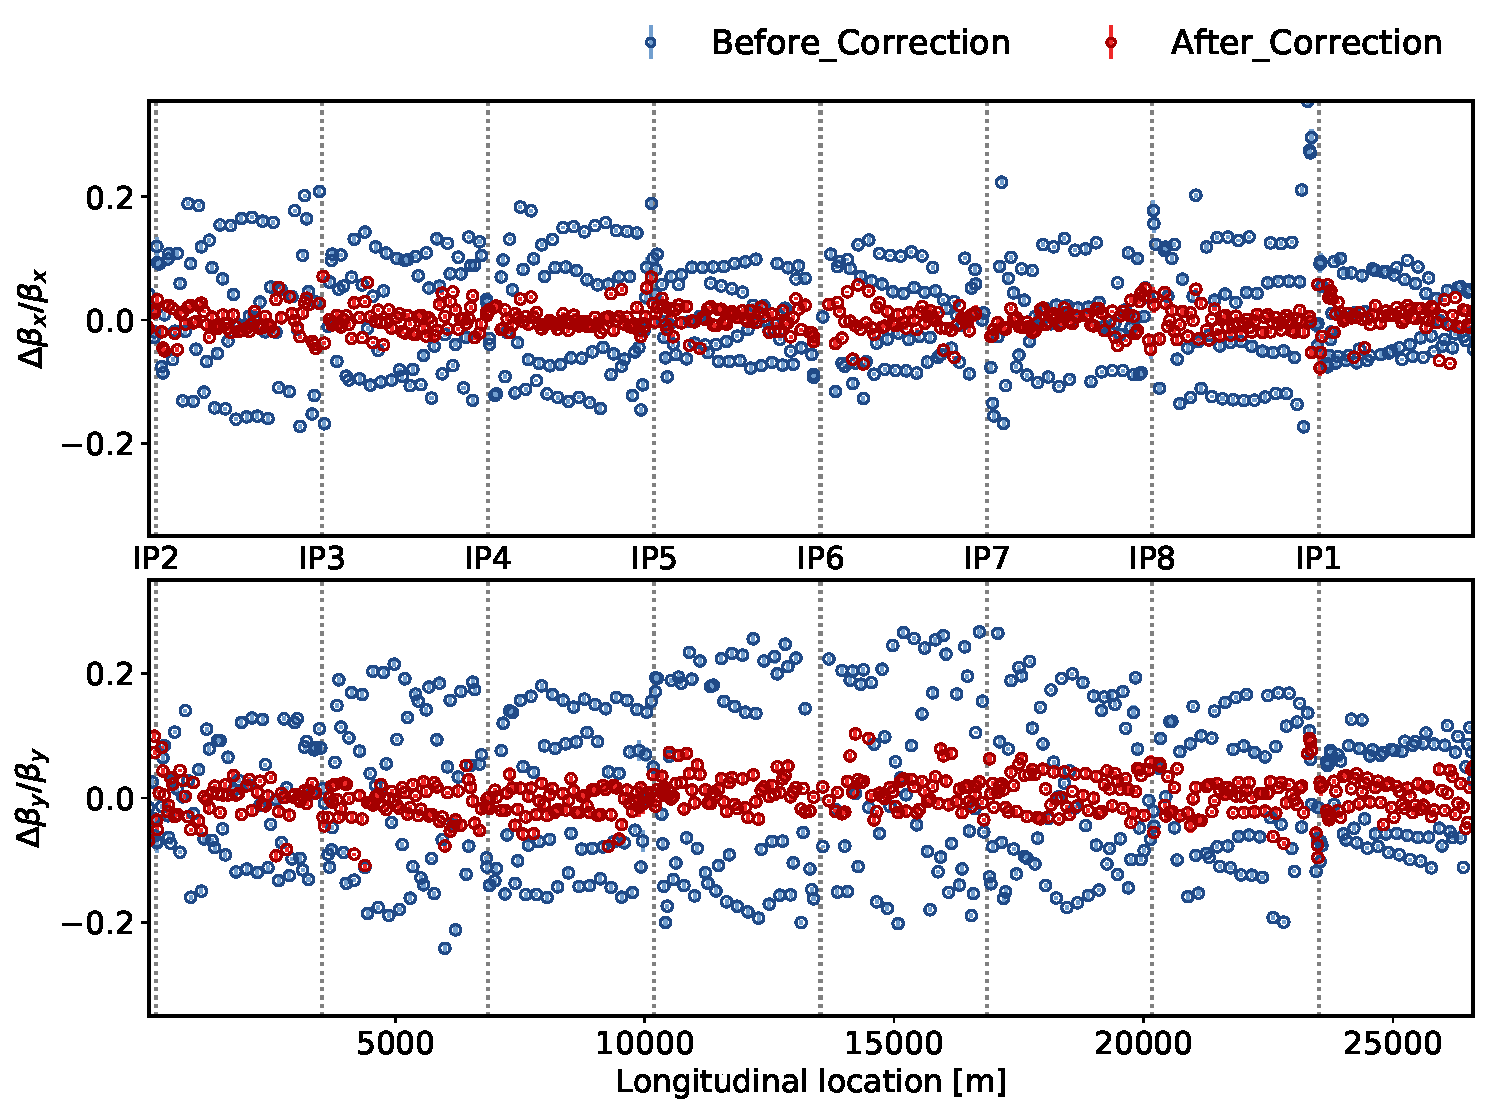
\includegraphics[width=.99\linewidth]{plots/beam1/beta_beat_before_and_after_corr.pdf}  
  \caption{Beam~1}
\end{subfigure}
\begin{subfigure}{.5\textwidth}
  \centering
  % include second image
  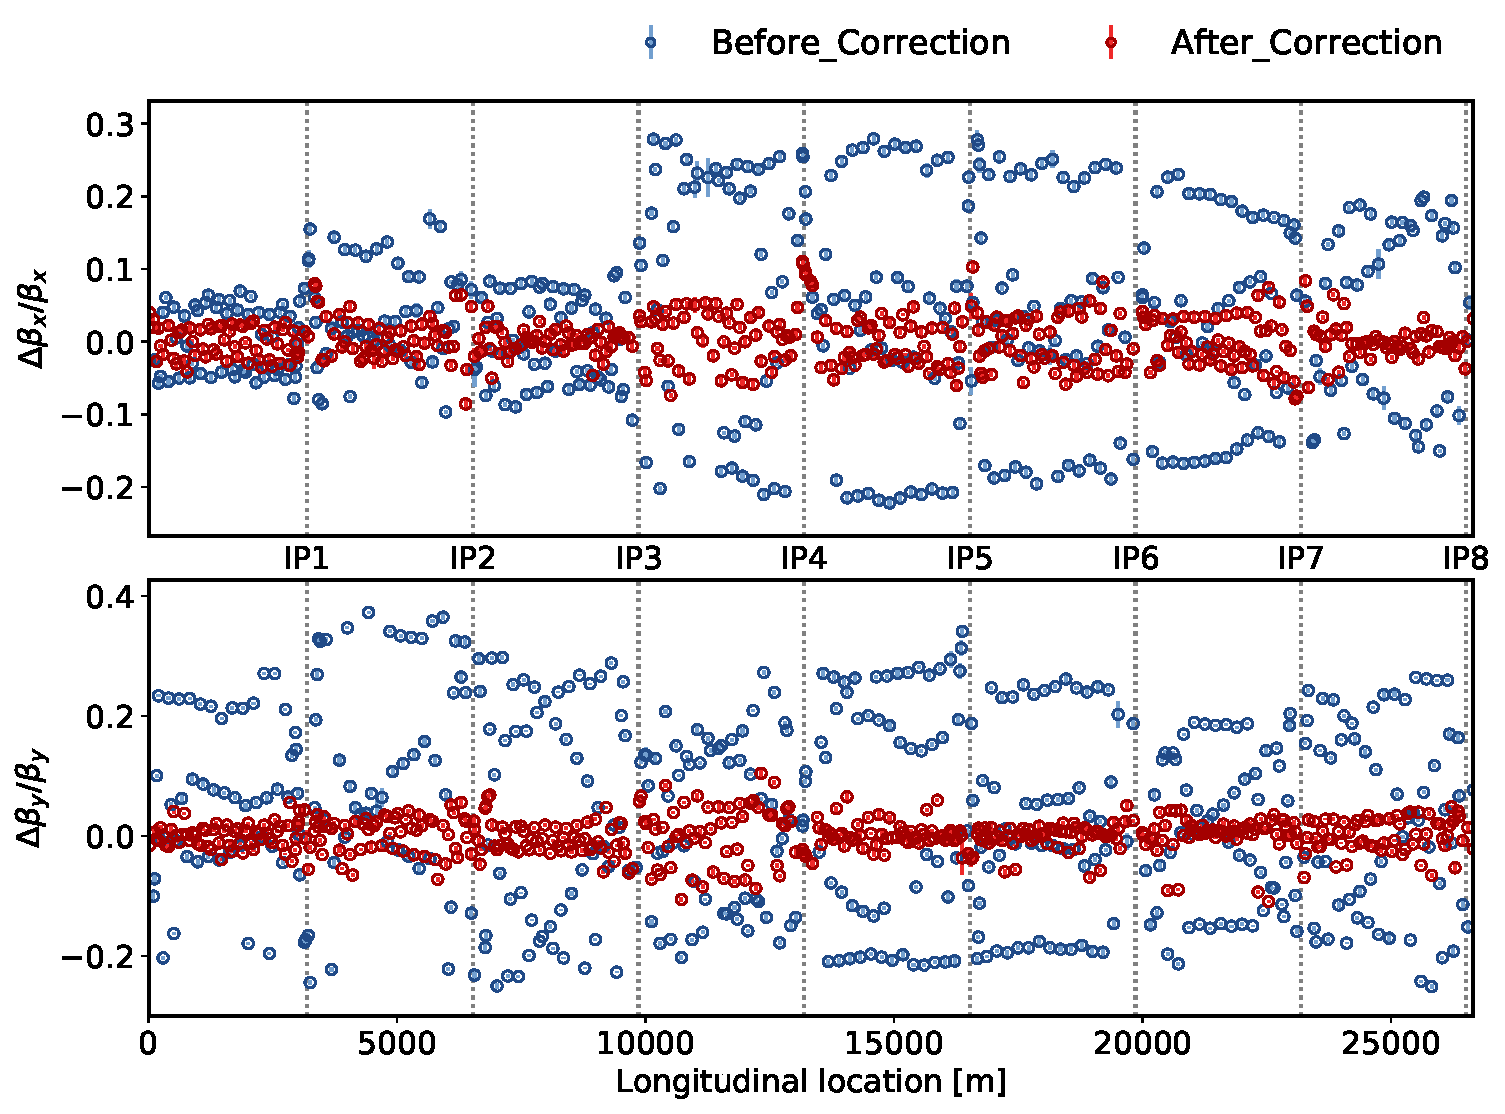
\includegraphics[width=.99\linewidth]{plots/beam2/beta_beat_before_after_correction.pdf}  
  \caption{Beam~2}
\end{subfigure}
\caption{Run 3 $\beta$-beating before and after correction.}
\label{fig:before_after_correction_beta_beat}
\end{figure}

\begin{figure}[ht]
\begin{subfigure}{.5\textwidth}
  \centering
  % include first image
  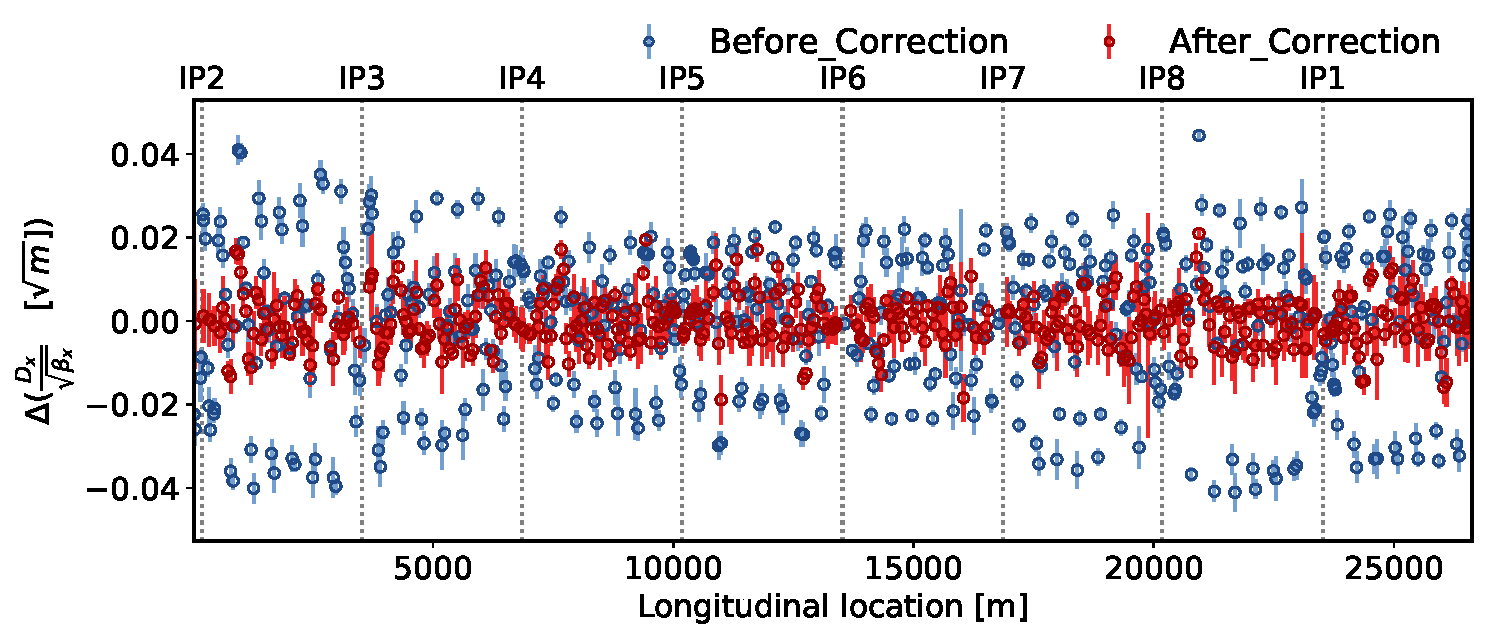
\includegraphics[width=.99\linewidth]{plots/beam1/Normalized_disp_before_vs_after_corection.pdf}  
  \caption{Beam~1}
\end{subfigure}
\begin{subfigure}{.5\textwidth}
  \centering
  % include second image
  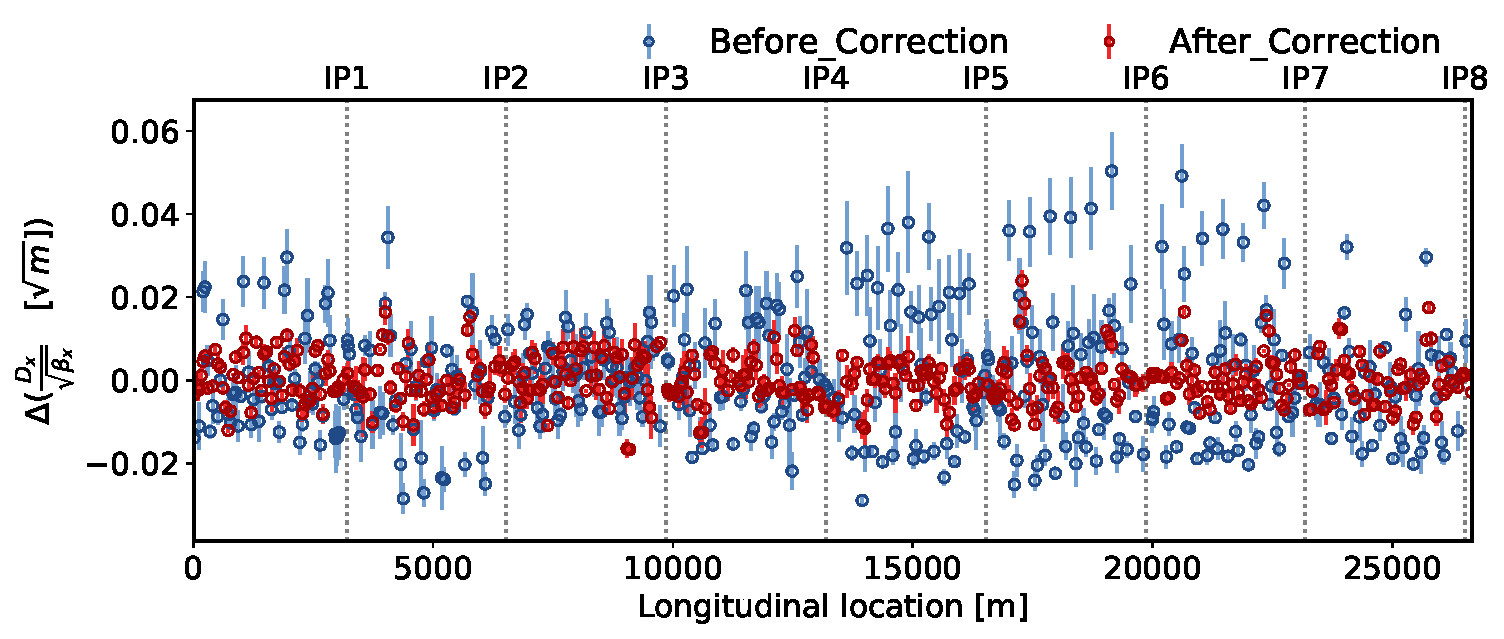
\includegraphics[width=.99\linewidth]{plots/beam2/ndisp_before_after_correction.pdf}  
  \caption{Beam~2}
\end{subfigure}
\caption{Normalized dispersion before and after correction in Run 3.}
\label{fig:before_after_correction_ndisp}
\end{figure}


Figure~\ref{fig:2017_beta_beat_vs_2021} shows a comparison of the $\beta$-beating in Run~2 cand Run~3 after global corrections. We can see that the level of corrections is similar for the two runs with a slight improvement for Beam~1 in Run~3. 

\begin{figure}[ht]
\begin{subfigure}{.5\textwidth}
  \centering
  % include first image
  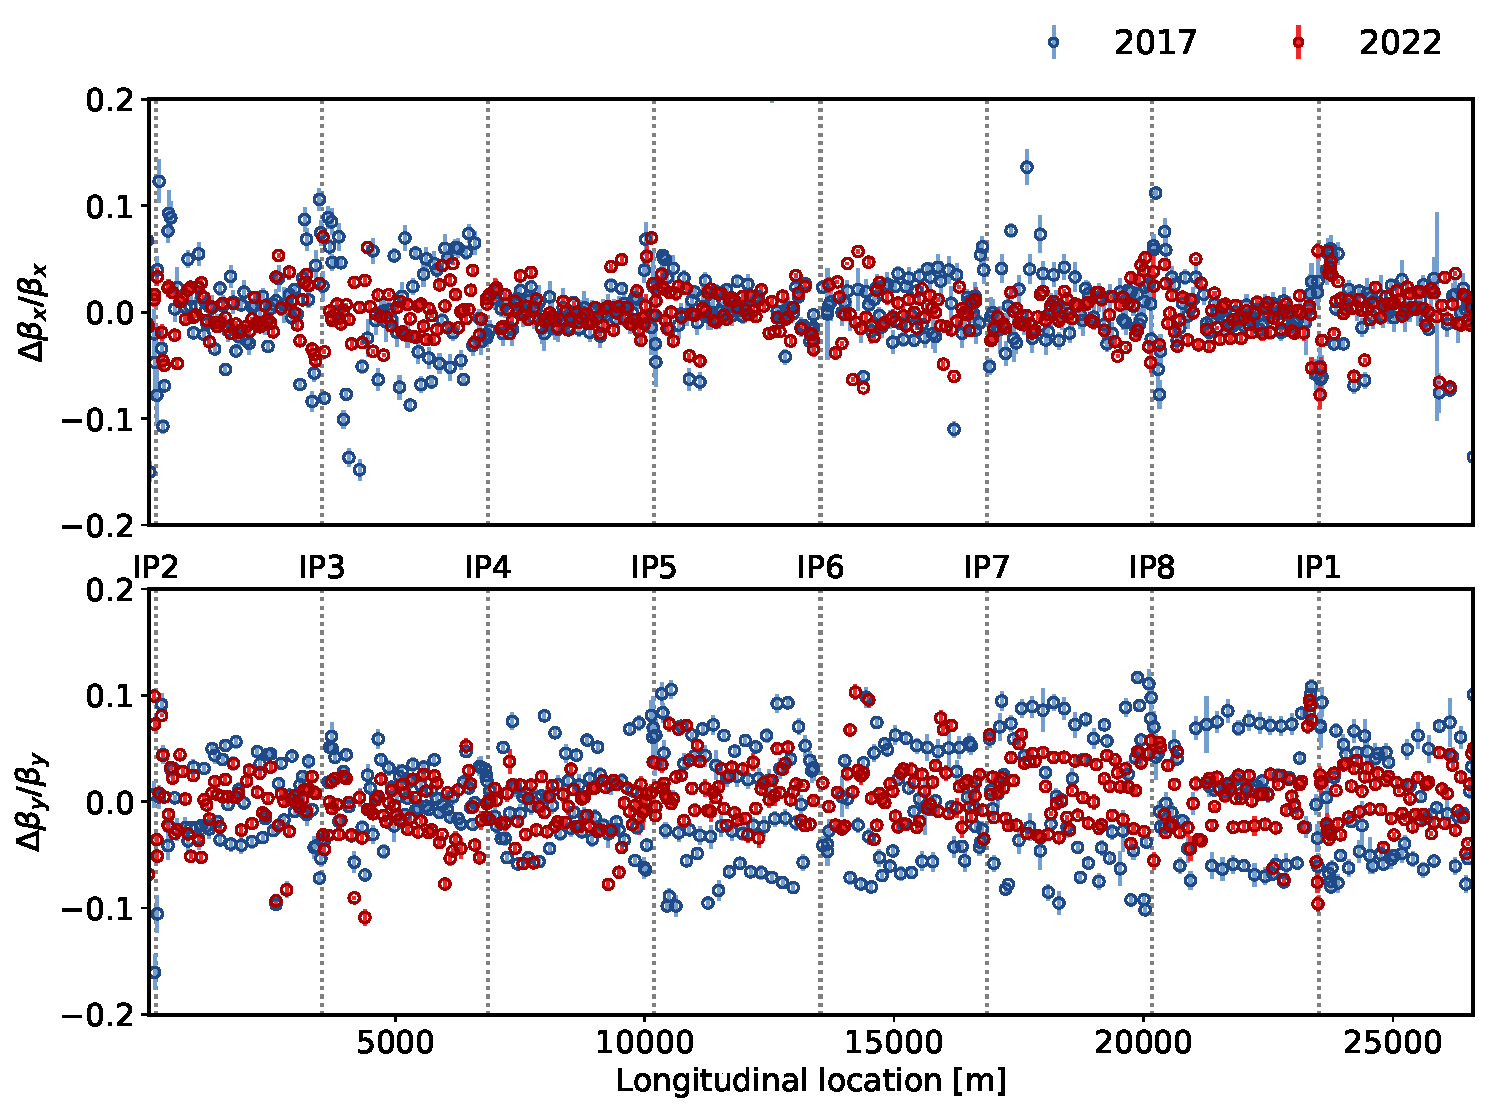
\includegraphics[width=.99\linewidth]{plots/beam1/after_corr_2017_vs_2021.pdf}  
  \caption{Beam~1}
\end{subfigure}
\begin{subfigure}{.5\textwidth}
  \centering
  % include second image
  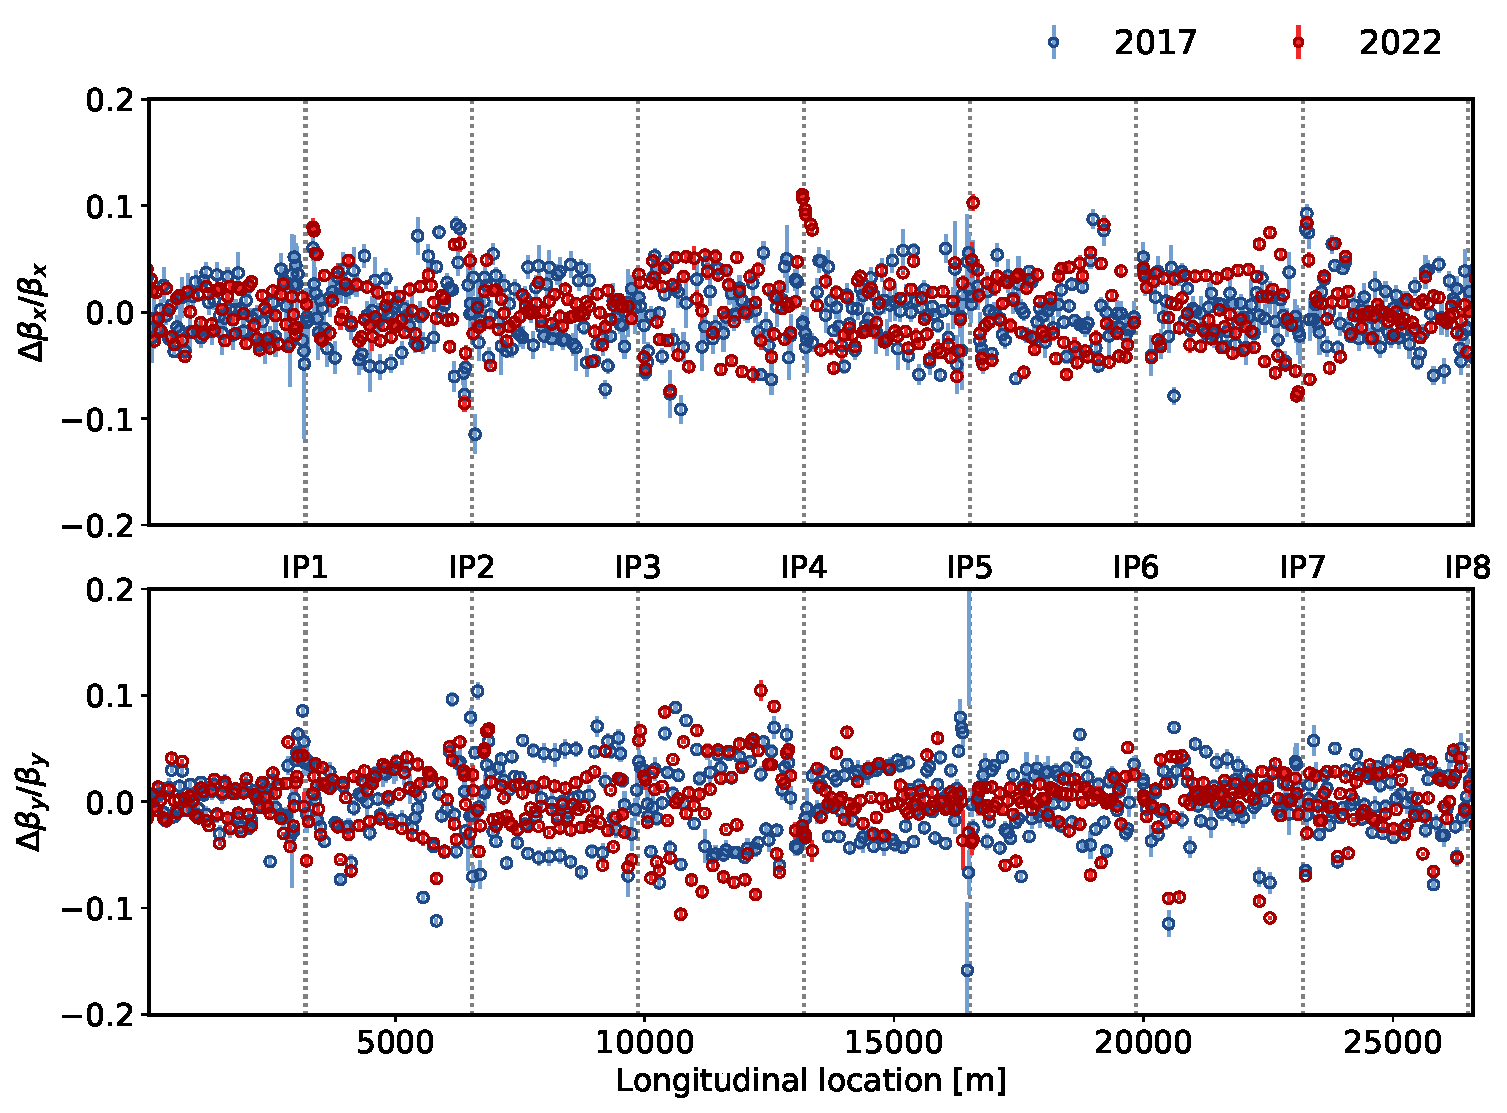
\includegraphics[width=.99\linewidth]{plots/beam2/after_corr_2017_vs_2021_beam2.pdf}  
  \caption{Beam~2}
\end{subfigure}
\caption{The $\beta$-beating measured after correction during the beam-test compared to what was measured at injection in 20107.}
\label{fig:2017_beta_beat_vs_2021}
\end{figure}

In Fig.~\ref{fig:corrector_strength_injection} the change in powering of the magnets to archive the corrections is shown. The maximum strength between the corrections used in Run~2 and Run~3 is very similar but fewer magnets were used for the Run~3 correction, in particular for Beam~1. This is due to slightly different settings being used to calculate the corrections.  

\begin{figure}[ht]
\begin{subfigure}{.5\textwidth}
  \centering
  % include first image
  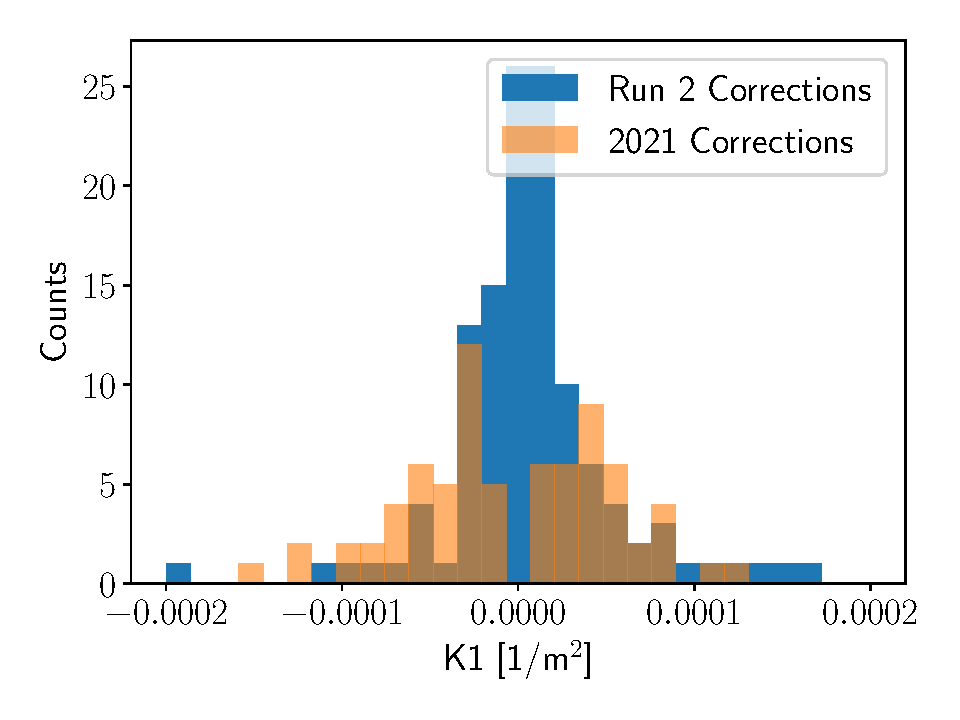
\includegraphics[width=.9\linewidth]{beam1_corrections.pdf}  
  \caption{Beam~1}
\end{subfigure}
\begin{subfigure}{.5\textwidth}
  \centering
  % include second image
  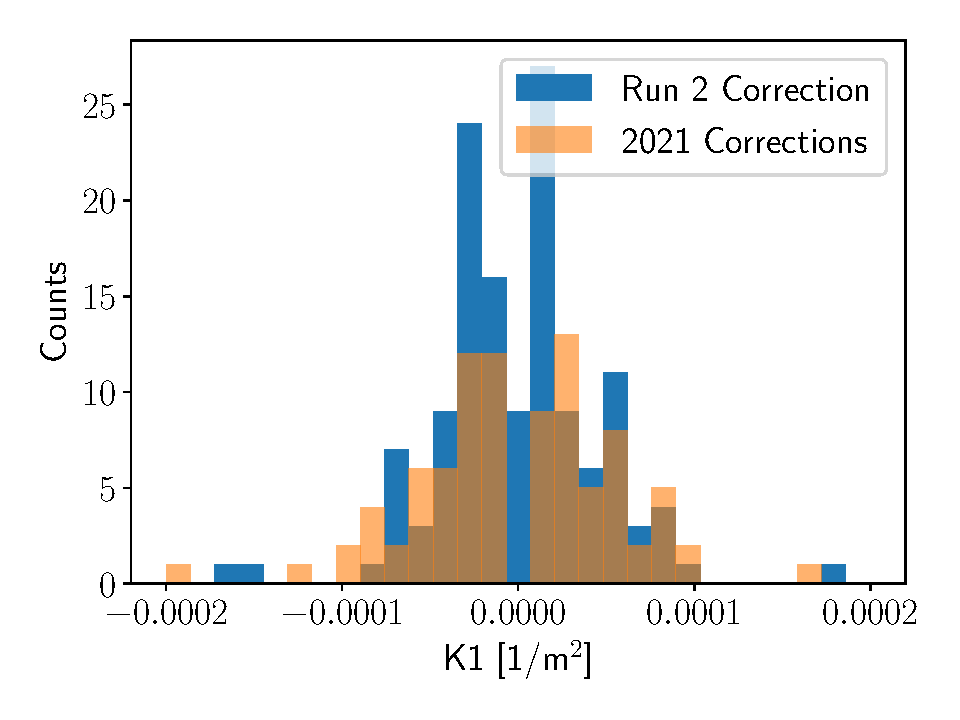
\includegraphics[width=.9\linewidth]{beam2_corrections.pdf}  
  \caption{Beam~2}
\end{subfigure}
\caption{The correction strengths used in Run~2 and Run~3.}
\label{fig:corrector_strength_injection}
\end{figure}



\subsection{Measurements in 2022 and reproducibility}\label{sec:repro}
No dedicated corrections were applied for the injections optics in 2022 but validation measurements were performed. Figure~\ref{fig:2021_beta_beat_vs_2022} shows a comparison of the $\beta$-beating measured during the beam test compared and the measurement in April 2022 at the beginning of the optics commissioning. We can observe that while Beam~1 seems to have similar $\beta$-beat values Beam~2 shows a slight increase. The increase was, however, small enough to not be considered to be an issue and was therefore left without any additional corrections. 


\begin{figure}[ht]
\begin{subfigure}{.5\textwidth}
  \centering
  % include first image
  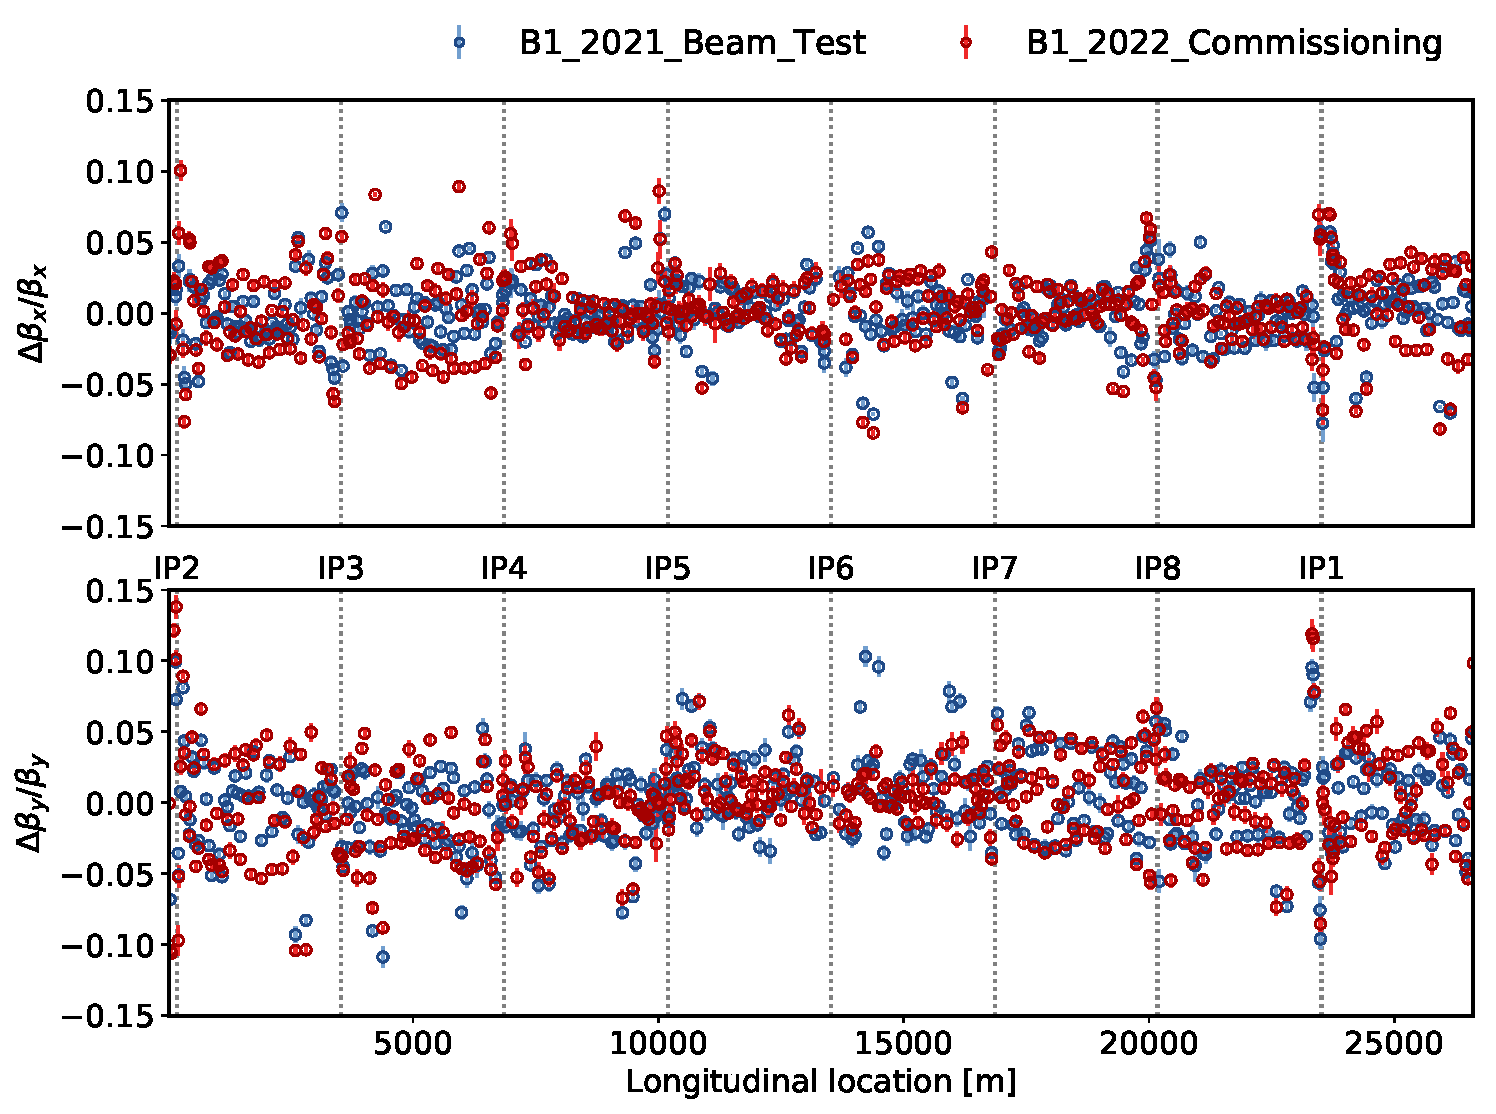
\includegraphics[width=.99\linewidth]{plots/beam1/lhcb1_betabeat_vs_beamtest.pdf}  
  \caption{Beam~1}
\end{subfigure}
\begin{subfigure}{.5\textwidth}
  \centering
  % include second image
  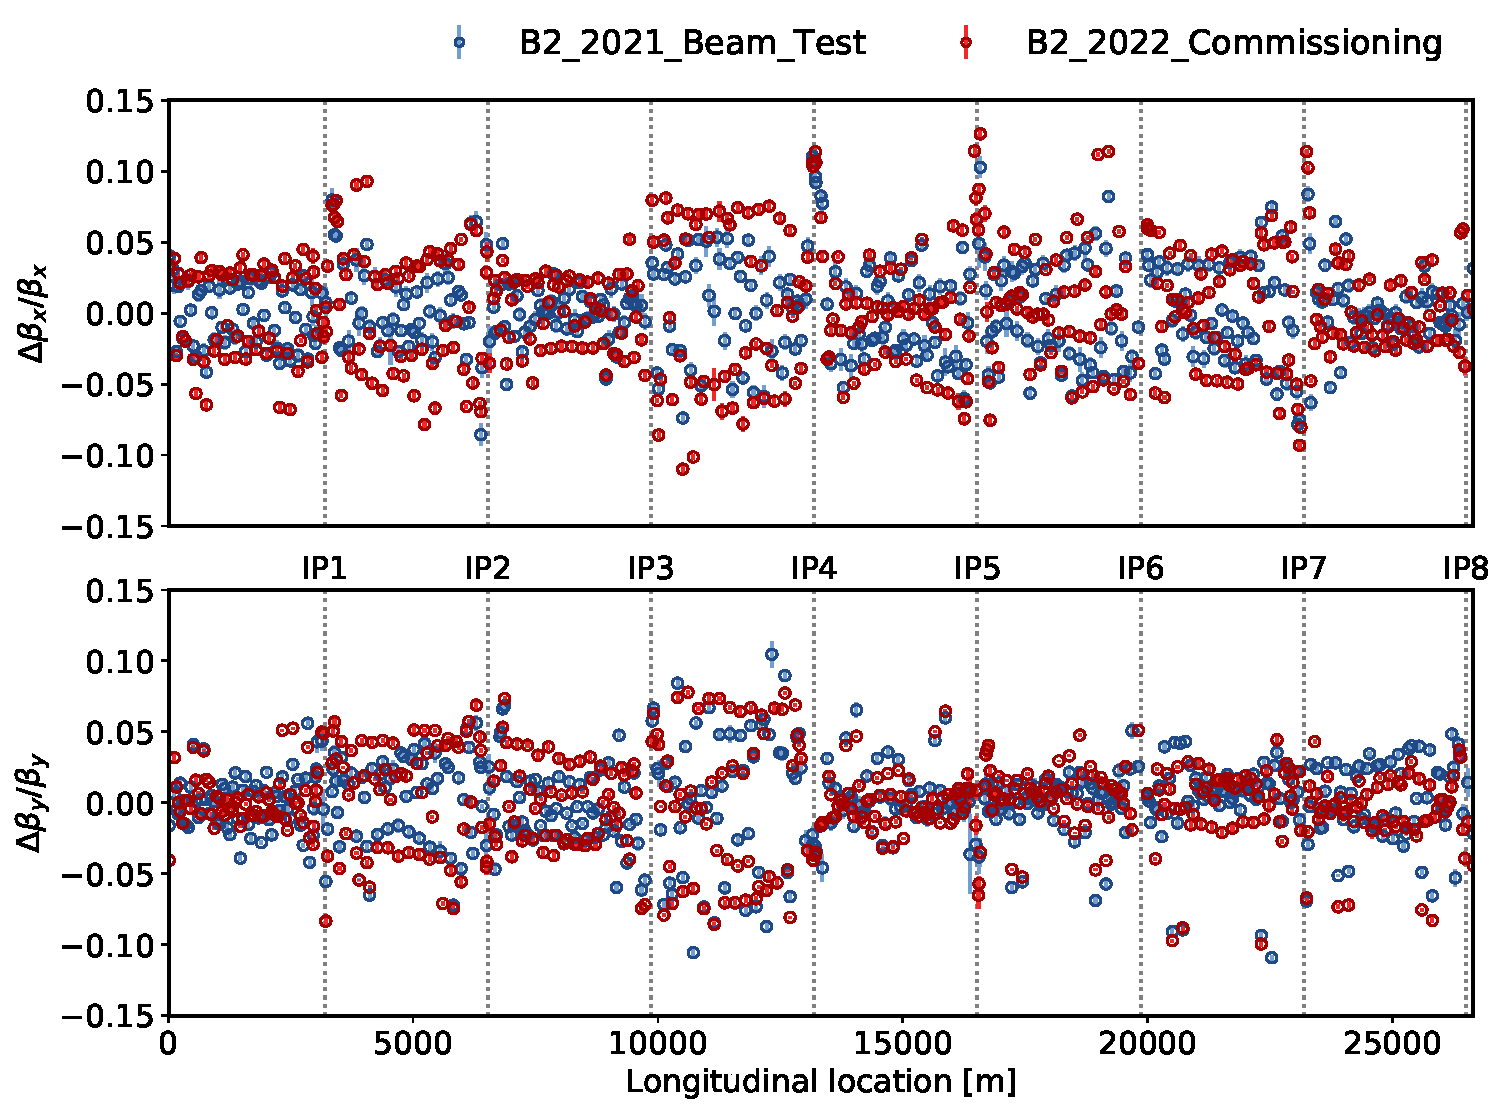
\includegraphics[width=.99\linewidth]{plots/beam2/lhcb2_betabeat_vs_beamtest.pdf}  
  \caption{Beam~2}
\end{subfigure}
\caption{The $\beta$-beating measured during the beam-test compared to what was measured at the beginning of the commissioning in 2022.}
\label{fig:2021_beta_beat_vs_2022}
\end{figure}
In order to understand the natural fluctuations of the $\beta$-beating
at injection, additional measurements were taken in parallel to other activities. In Fig.~\ref{fig:comp_several_beam2} we observe that the $\beta$-beat varies by a few percent depending on the measurement. The energy at the LHC is sometimes slightly adjusted to be matched to the energy of the SPS by changing the average strength of the horizontal corrector magnets. The typical fluctuations are within a few $10^{-4}$. A study which simulated this effect could rule out this as being the cause of the change, as seen in~Fig.~\ref{fig:energy_offset_injection}.

\begin{figure}
  \centering
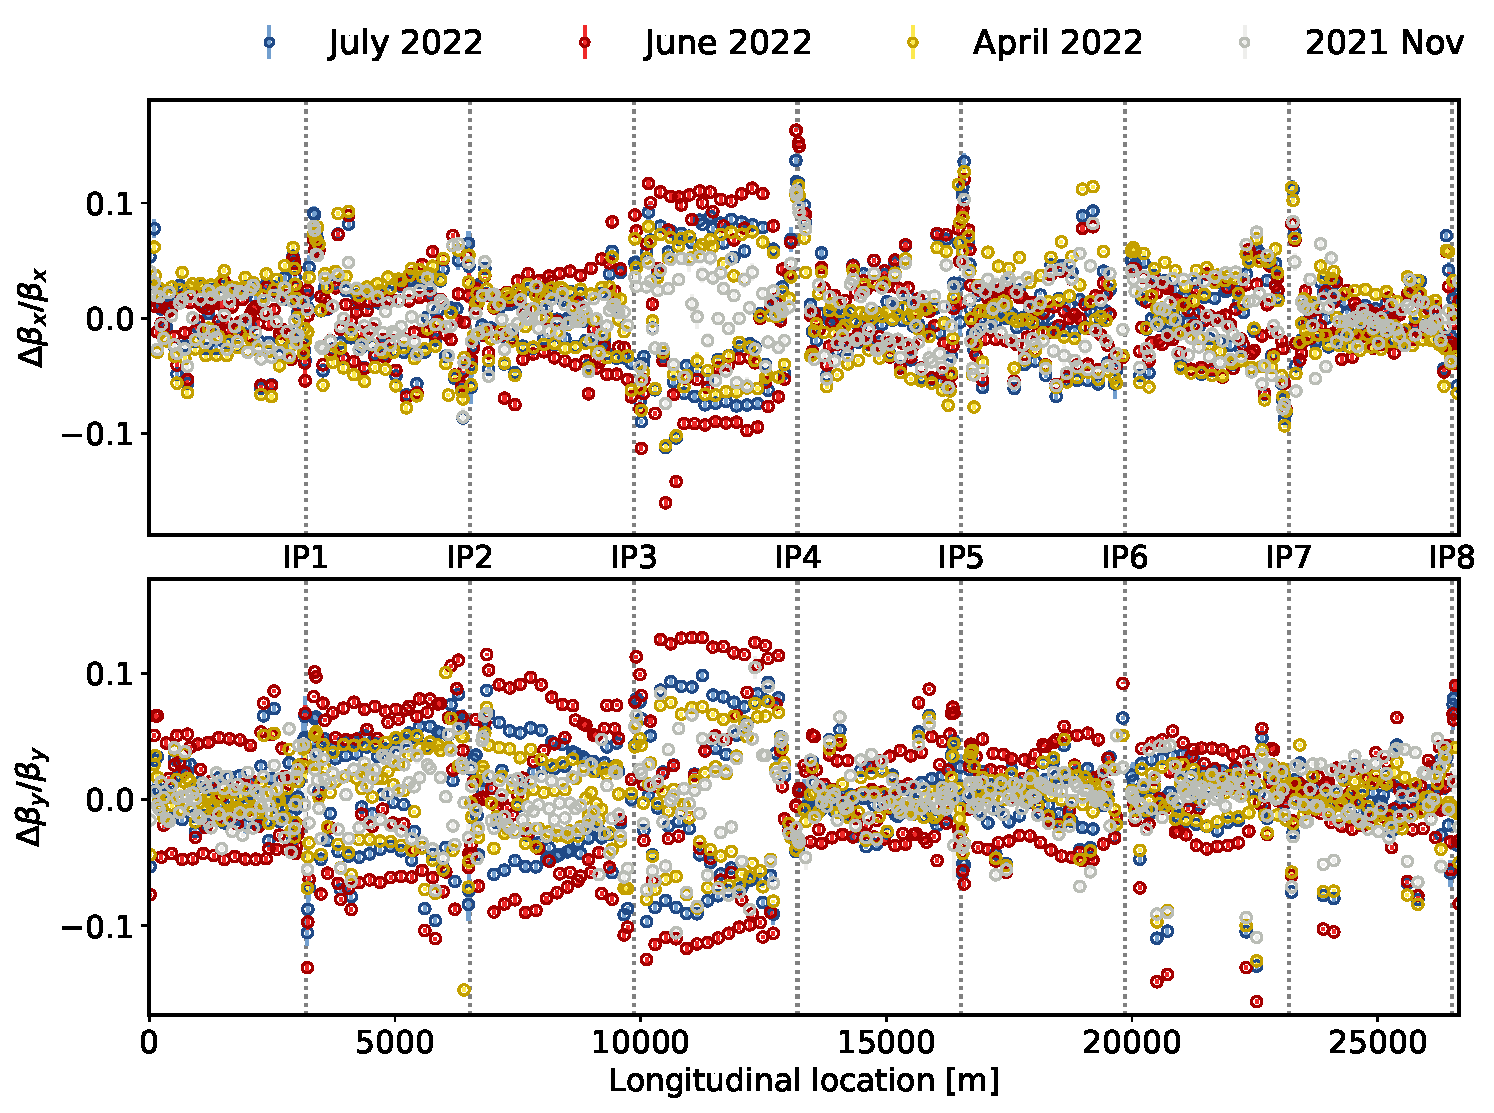
\includegraphics[width=0.8\linewidth]{plots/beam2/comp_injection_several.pdf}
\caption{Beam 2 $\beta$-beating measured at injection on several different occasions during 2021 and 2022. }
\label{fig:comp_several_beam2}
\end{figure}

\begin{figure}
  \centering
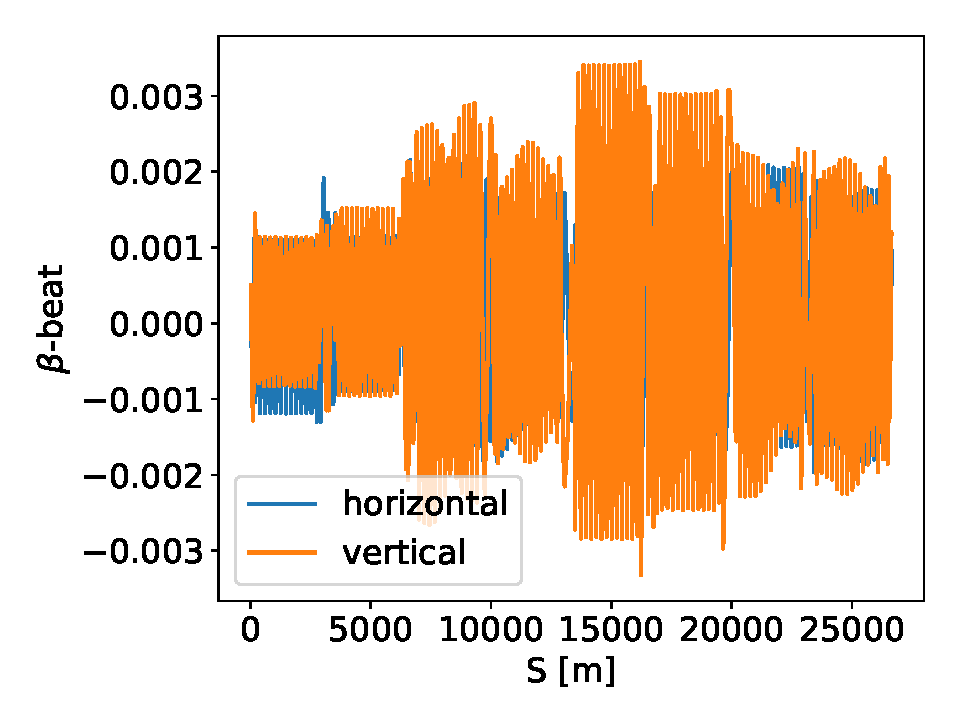
\includegraphics[width=0.8\linewidth]{plots/beam2/injection_energy.pdf}
\caption{The change in $\beta$-beating of Beam 2 from introducing an energy offset of $10^{-4}$ at injection. }
\label{fig:energy_offset_injection}
\end{figure}

The variation is within the tolerance where it is not an issue for machine protection. 


\begin{comment}

\clearpage
\section{Q'' and Q''' measurements}

Two attempts were made during the beam-test to measure the chromaticity. The first attempt was successful while the second one only was a half scan, resulting in non exploitable data. Moreover, corrections were done for this second measurement assuming last run's values.\\
The times below are local times.

\begin{longtable}[h]{l l}
  \toprule
  \textbf{Beam Process}: & SPOOLS-6.8TeV-2021\_V1@0\_[START]\\
  \textbf{Date}: & 2021-10-22 \\
  \textbf{Start Time}: & 16:05:30\\
  \textbf{End Time}: & 16:37:00\\
  \textbf{dpp range:} & -0.0027 to +0.0017 \\
  \bottomrule
  \caption{First Measurement}
\end{longtable}

\begin{longtable}[h]{l l}
  \toprule
  \textbf{Beam Process}: & SPOOLS-6.8TeV-2021\_V1@0\_[START]\\
  \textbf{Date}: & 2021-10-31\\
  \textbf{Start Time}: & 12:16:00\\
  \textbf{End Time}: & 12:30:00 \\
  \textbf{dpp range:} & -0.0033 to +0.00\\
  \midrule
  \textbf{MCO Strengths}: & B1/B2: +3.9 / +2.7 \\
  \textbf{MCD Strengths}: & B1/B2: +2316 / +2053 \\
  \bottomrule
  \caption{Second Measurement}
\end{longtable}

% Plots for Beam 1, first axis X, then Y
\begin{figure}[H]
  \centering
  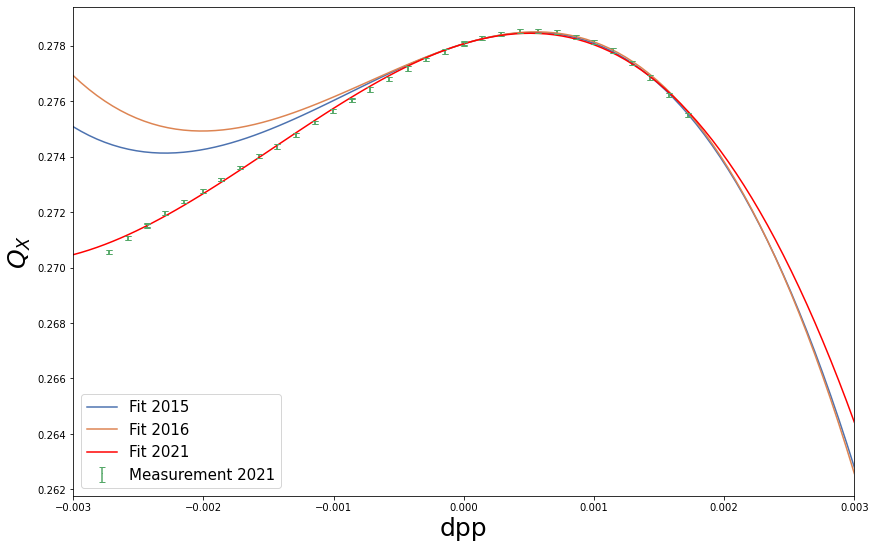
\includegraphics[width=.8\linewidth]{plots/beam1/qxb1.png}  
  \caption{Chromaticity on the X axis for Beam 1}
\end{figure}
\begin{figure}[H]
  \centering
  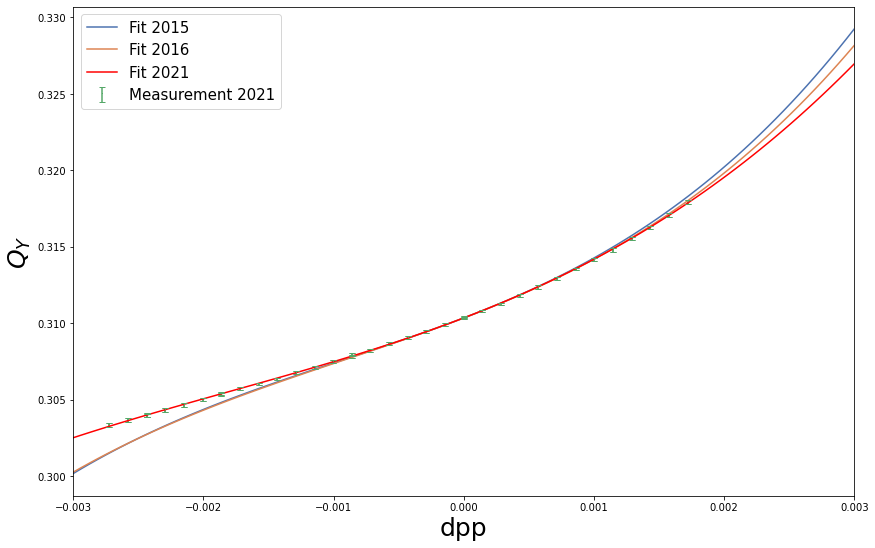
\includegraphics[width=.8\linewidth]{plots/beam1/qyb1.png}  
  \caption{Chromaticity on the Y axis for Beam 1}
\end{figure}

% Plots for Beam 2, first axis X, then Y
\begin{figure}[H]
  \centering
  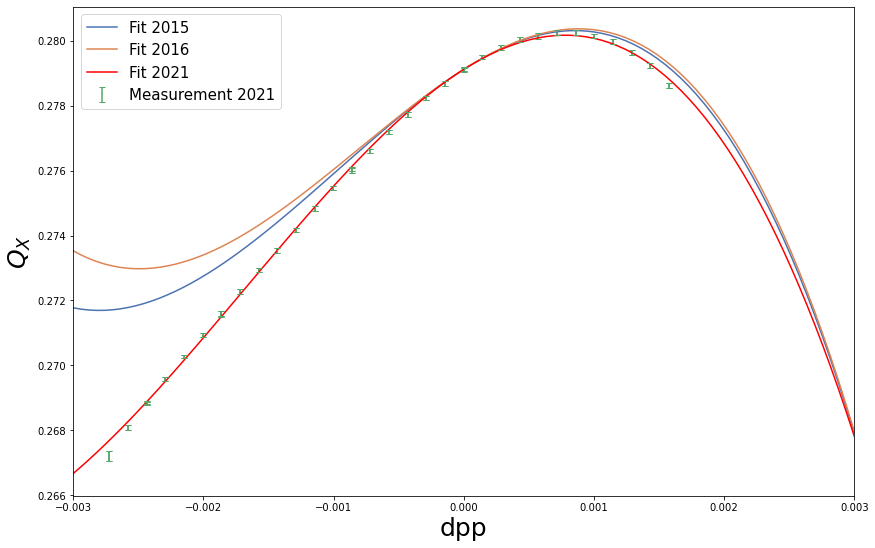
\includegraphics[width=.8\linewidth]{plots/beam2/qxb2.png}  
  \caption{Chromaticity on the X axis for Beam 2}
\end{figure}
\begin{figure}[H]
  \centering
  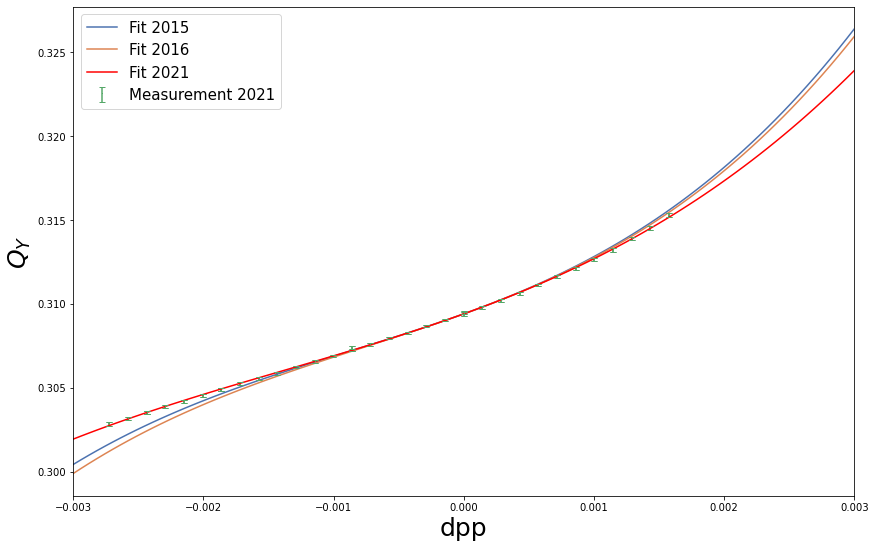
\includegraphics[width=.8\linewidth]{plots/beam2/qyb2.png}  
  \caption{Chromaticity on the Y axis for Beam 2}
\end{figure}

\begin{longtable}[h]{@{}l|c|rr|rr@{}}
  \toprule
  Year & Beam & $Q_x''[10^3]$ &   $Q_x'''[10^6]$ &   $Q_y''[10^3]$ &  $Q_y'''[10^6]$ \\
  \midrule
  \endhead
  2011 &   B1 &   $-1.8 \pm 0.03$ &  $-2.2 \pm 0.1$ &   $0.86 \pm 0.02$ &   $0.73 \pm 0.07$ \\
       &   B2 &   $-1.7 \pm 0.05$ &  $-1.1 \pm 0.1$ &   $0.82 \pm 0.02$ &   $0.90 \pm 0.06$ \\
  \midrule
  2015 &   B1 &   $-2.03 \pm 0.02$ &  $-2.31 \pm 0.08$ &   $0.97 \pm 0.02$ &   $1.06 \pm 0.04$ \\
       &   B2 &   $-2.06 \pm 0.02$ &  $-2.12 \pm 0.05$ &   $0.89 \pm 0.01$ &   $1.02 \pm 0.02$ \\
  \midrule
  2016 &   B1 &   $-1.85 \pm 0.03$ &  $-2.54 \pm 0.07$ &   $0.86 \pm 0.01$ &   $0.93 \pm 0.04$ \\
       &   B2 &   $-1.86 \pm 0.02$ &  $-2.31 \pm 0.05$ &   $0.78 \pm 0.01$ &   $1.03 \pm 0.05$ \\
  \midrule
  2021 &   B1 &   $-2.36 \pm 0.03$ &  $-1.62 \pm 0.04$ &  $0.98 \pm 0.01$ &  $0.55 \pm 0.02$ \\
       &   B2 &   $-2.64 \pm 0.03$ &  $-1.56 \pm 0.05$ &  $0.78 \pm 0.01$ &   $0.58 \pm 0.02$ \\
  \bottomrule
  \caption{Non Linear Chromaticity Results and History}
\end{longtable}

\end{comment}

\section{MCS feed-down}
It has been observed that changing the strength of the MCSs ($b_3$ spool pieces) has an impact on the transverse coupling in the LHC~\cite{counter_acting_coupling_decay}. The main hypothesis is that this is coming from a vertical misalignment of the MCS with respect to the $b_3$ in the main dipoles or from a systematic orbit effect. In order to validate if the effect had remained constraint after LS2 a new measurement was carried out during the beam-test. The test consists of adjusting the setting of the MCS in a single arc and measuring the impact on the transverse coupling. The result for Beam~1 is shown in Fig.~\ref{fig:beam1_mcs} and for Beam~2 in  Fig.~\ref{fig:beam2_mcs}. Beam~1 has fewer measurements since the MD in 2018 was only for Beam~2. We observe that both the amplitude and the sign seem to have stayed constant between Run~2 and Run~3. This is an important observation since this indicates that the coupling feed-down caused by this could be mitigated as proposed in \cite{counter_acting_coupling_decay}. In fact, the proposal to compensate for the dynamic part of the $b_3$-decay was implemented in 2022 showing promising results but a final analysis of the impact of this will be reported in a future report.
%Add reference here

\begin{figure}[ht]
\begin{subfigure}{.5\textwidth}
  \centering
  % include first image
  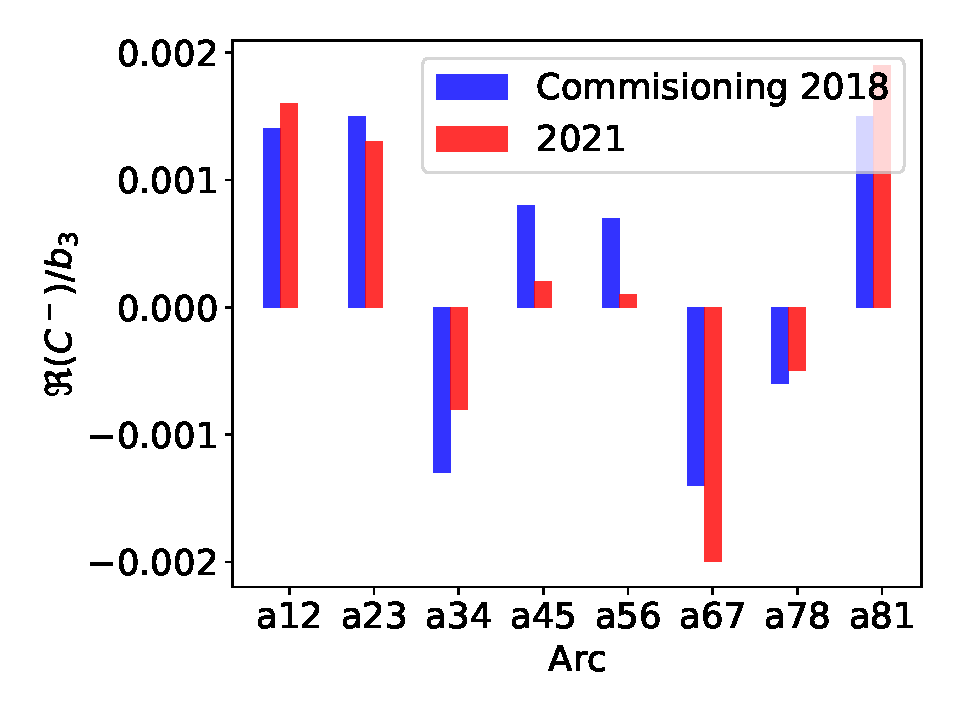
\includegraphics[width=.8\linewidth]{plots/MCS/b_1change_re_per_b3.pdf}  
  \caption{Real part of the $C^-$.}
\end{subfigure}
\begin{subfigure}{.5\textwidth}
  \centering
  % include second image
  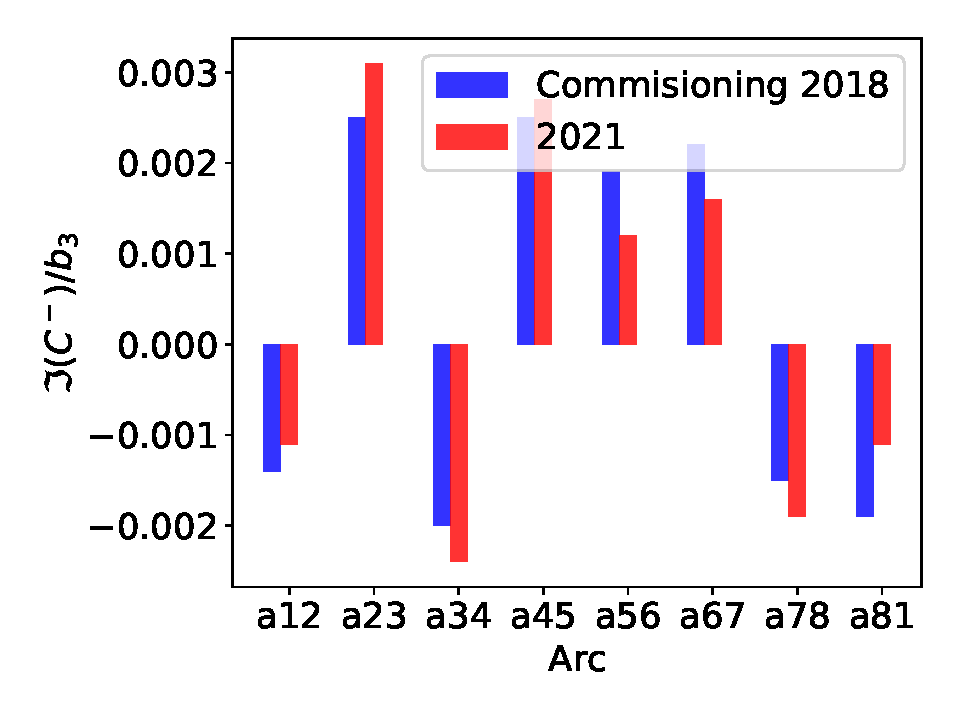
\includegraphics[width=.8\linewidth]{plots/MCS/b_1change_im_per_b3.pdf}  
  \caption{Imaginary part of the $C^-$.}
\end{subfigure}
\caption{The impact on the $C^-$ from changing the MCS corrector ($b_3$-spool pieces) for Beam~1. }
\label{fig:beam1_mcs}
\end{figure}

\begin{figure}[ht]
\begin{subfigure}{.5\textwidth}
  \centering
  % include first image
  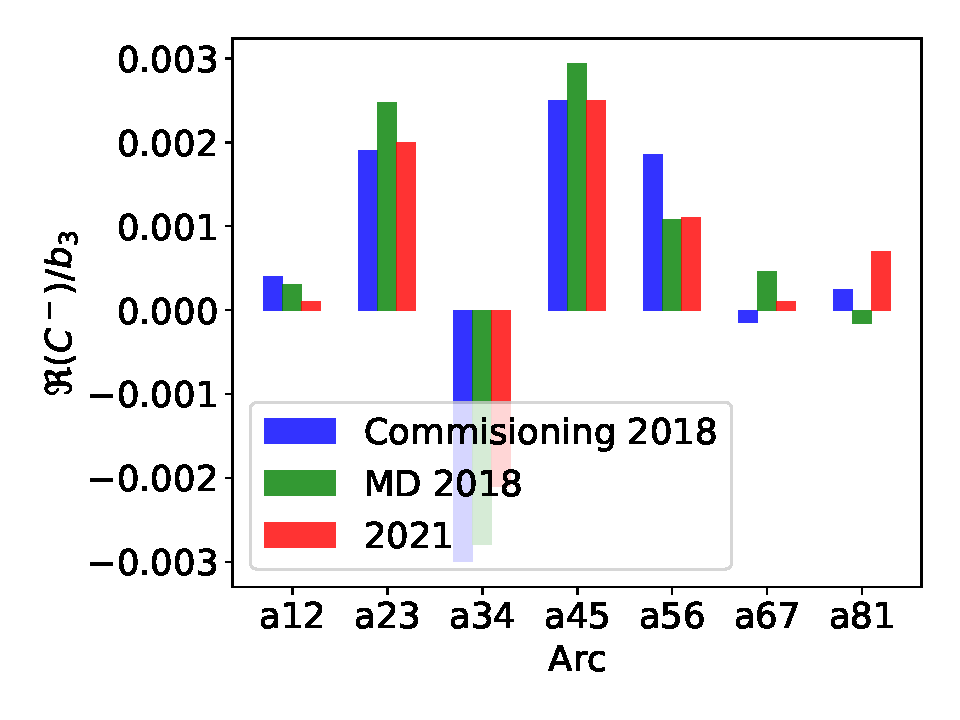
\includegraphics[width=.8\linewidth]{plots/MCS/b2_change_re_per_b3.pdf}  
  \caption{Real part of the $C^-$.}
\end{subfigure}
\begin{subfigure}{.5\textwidth}
  \centering
  % include second image
  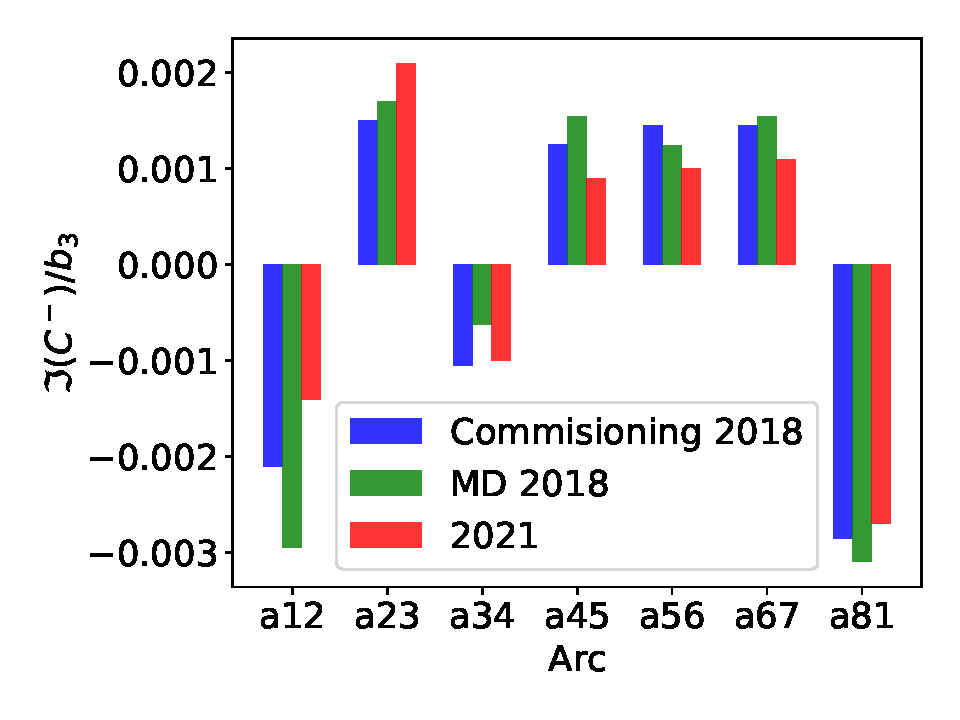
\includegraphics[width=.8\linewidth]{plots/MCS/b_2change_im_per_b3.pdf}  
  \caption{Imaginary part of the $C^-$.}
\end{subfigure}
\caption{The impact on the $C^-$ from changing the MCS corrector ($b_3$-spool pieces) for Beam~1.}
\label{fig:beam2_mcs}
\end{figure}


\section{Summary and Outlook}
The optics corrections during the beam test were successful in terms of demonstrating the readiness of the optics corrections tools as well as finding the swap of the magnets RQTL7.R3.B1 $\leftrightarrow$ RQTL7.R3.B2. Furthermore, it was very useful in testing the tools and software packages to be ready for Run~3. The optics corrections also remained the same for the 2023 Run. A degradation of the optics quality was observed for Beam~2 but not for Beam~1. Through simulations, it has been excluded to derive from energy variations at injection. Instead, it is more likely that it derives from hysteresis or/and decays at injection. It would be interesting to measure the optics at different intervals over a longer time period. This could potentially be combined with a scrubbing run where one could apply kicks between the fills for scrubbing. Additionally, it would be interesting to understand if there is a difference between a pre-cycle and a ramp-down. 

\begin{thebibliography}{99}   % Use for  1-9  reference

\bibitem{ats_stephane}
S.~Fartoukh, ``Achromatic telescopic squeezing scheme and its application to the LHC and its luminosity upgrade'', Phys. Rev. ST Accel. Beams {\bf16}, 111002 (2013)

\bibitem{roderik} R. Bruce, {\it et al.}, ``New IR7 optics with removed
MQW magnets'',  \href{https://indico.cern.ch/event/681507/contributions/2814548/attachments/1570845/2478033/2017.12.06--HSS_meeting_MQW_removal.pdf}{ABP-HSS Section meetings,
Wednesday 6 Dec. 2017}.


\bibitem{LS2} S. Le Naour, ``LS2 magnet modifications'', LS2 Powering Test- Preparation day, 17 Nov. 2020,
\url{https://indico.cern.ch/event/967907/contributions/4084438/attachments/2144305/3613896/2020-11-17_LS2PoweringTest.pdf}

\bibitem{LS2a} A. Apollonio, {\it et al.}, ``SUMMARY OF THE POST-LONG SHUTDOWN 2
LHC HARDWARE COMMISSIONING CAMPAIGN'', IPAC 2022,  \url{doi:10.18429/JACoW-IPAC2022-MOPOPT040}.

\bibitem{run3} S. Fartoukh, {\it et al.}, 
	``LHC Configuration and Operational Scenario for Run 3'', CERN-ACC-2021-0007.
\bibitem{first} M. Aiba, S. Fartoukh, A. Franchi, M. Giovannozzi, V. Kain, M. Lamont, R. Tom\'as, G. Vanbavinckhove, J. Wenninger, F. Zimmermann, R. Calaga, and A. Morita, ``First beta-beating measurement and optics analysis for the CERN Large Hadron Collider'', Phys. Rev. ST Accel. Beams {\bf12}, 081002 (2009).

\bibitem{michiEvian}  M.~Hostettler, ``The 2021 beam test results and lessons learned'', Evian OP Workshop 2021, CERN, Switzerland
\url{https://indico.cern.ch/event/1077835/contributions/4533367/attachments/2350863/4009681/2021_Evian_BeamTest.pdf}

\bibitem{counter_acting_coupling_decay} T.~Persson, {\it et al.},  ``LHC 3324: Counteracting coupling decay at injection'', \url{https://cds.cern.ch/record/275393}

\end{thebibliography}
\begin{comment}


\appendix
\section{Decay compensation}
Based on the measurement of the feed-down from the MCS to coupling a new powering to compensate for the b3 decay in the dipoles have been calculated. It is matched in such a way that it compensates the chromaticity by the same amount as the even compensation but distributed in such a way that the coupling is expected to stay constant. The knobs for this are the following:
\begin{verbatim}

RCS.A12B1/K2 0.8630127907663837 
RCS.A23B1/K2 0.779866457813889 
RCS.A34B1/K2 1.3828734821095998 
RCS.A45B1/K2 0.4445174033278492 
RCS.A56B1/K2 0.9114975331776818 
RCS.A67B1/K2 1.401218693590656 
RCS.A78B1/K2 1.3540008484475567 
RCS.A81B1/K2 0.8630127907663839 

RCS.A12B2/K2 0.6866554457561092 
RCS.A23B2/K2 0.9619053275562472 
RCS.A34B2/K2 1.5867931783979445 
RCS.A45B2/K2 0.7923501971731068 
RCS.A56B2/K2 0.9643136781336532 
RCS.A67B2/K2 1.391600462298758 
RCS.A78B2/K2 1.16296351210475 
RCS.A81B2/K2 0.5945946691676663 

\end{verbatim}
\end{comment}
\end{document}
